\documentclass[11pt]{article}
\usepackage[letterpaper,hmargin=3cm,vmargin=3cm]{geometry}
\usepackage{amssymb,amsmath,amsfonts,eurosym,geometry,ulem,caption, subcaption,color,setspace,sectsty,comment,footmisc,pdflscape,subfig,array}
%\usepackage{palatino,amssymb,amsfonts,amsmath,latexsym,setspace}
\usepackage{utopia,latexsym}
\PassOptionsToPackage{pdftex}{graphicx}
\usepackage{graphicx}
\captionsetup{justification=centering}
\usepackage{fancyhdr}
\usepackage[dvipsnames]{xcolor}
\usepackage[utf8]{inputenc}
\usepackage[T1]{fontenc}
\usepackage{dutchcal}
\usepackage{amsthm}
\usepackage{booktabs}
\usepackage{float}
\usepackage{lscape}
\usepackage{eurosym}
\usepackage[font=footnotesize,labelfont=bf]{caption}
\usepackage{dcolumn}
\usepackage{booktabs}
\usepackage[dvipsnames]{xcolor}
\usepackage[authoryear]{natbib}
\usepackage{adjustbox}
\usepackage{microtype}
\usepackage{array}
\usepackage{siunitx}
\usepackage{threeparttable, multirow}
%\usepackage{hyperref}
\usepackage{listings}
\usepackage[most]{tcolorbox}

 \aboverulesep=0ex %make vertical lines continuous when needed.
 \belowrulesep=0ex %make vertical lines continuous when needed. 


\usepackage{appendix}
\appendixtitleon


\usepackage{tikz}
\let\latextable\table
\renewcommand\table[1][]{\latextable[H]}
\normalem

\def\checkmark{\tikz\fill[scale=0.4](0,.35) -- (.25,0) -- (1,.7) -- (.25,.15) -- cycle;} 

\definecolor{blue_citations}{HTML}{08088A}

\usepackage{adjustbox} %for adjusting tables width


\usepackage[colorlinks=true,linkcolor=black,citecolor=blue_citations,urlcolor=Violet,breaklinks]{hyperref}


\usetikzlibrary{decorations.pathreplacing,angles,quotes}
\usepackage[labelsep=period,font=small,textfont=bf,labelfont=bf,skip=0.1cm]{caption}
%\usepackage[labelformat=simple,labelsep=period,font=small,skip=0.0cm]{subcaption}
\setlength{\parskip}{2mm}
\newtheorem{theorem}{Theorem}
\newtheorem{corollary}[theorem]{Corollary}
\newtheorem{proposition}{Proposition}
\newtheorem{hypothesis}{Hypothesis}
\newtheorem{result}{Result}
\newtheorem{assumption}{Assumption}
\newtheorem{observation}{Observation}
\newtheorem{lemma}{Lemma}
\newtheorem{definition}{Definition}



\newtheorem{hyp}{Hypothesis}
\newtheorem{subhyp}{Hypothesis}[hyp]
\renewcommand{\thesubhyp}{\thehyp\alph{subhyp}}

\newcommand{\red}[1]{{\color{red} #1}}
\newcommand{\blue}[1]{{\color{blue} #1}}

\newcolumntype{L}[1]{>{\raggedright\let\newline\\arraybackslash\hspace{0pt}}m{#1}}
\newcolumntype{C}[1]{>{\centering\let\newline\\arraybackslash\hspace{0pt}}m{#1}}
\newcolumntype{R}[1]{>{\raggedleft\let\newline\\arraybackslash\hspace{0pt}}m{#1}}

% Command for better table alignment
\newcommand\mc[1]{\multicolumn{1}{c}{#1}} % handy shortcut macro


% Fix title, sections, etc.

\let\LaTeXtitle\title
\renewcommand{\title}[1]{\LaTeXtitle{{\LARGE #1}}}



  
 

\newcommand{\ri}{r_i}
\newcommand{\rj}{r_j}
\newcommand{\cbar}{\bar{c}}


\newcommand{\dstirling}[2]{\genfrac{}{}{0pt}{0}{#1}{#2}}


\begin{document}
\begin{sloppypar}

%==============================================================================
%This is the title page
\setcounter{page}{1} \thispagestyle{empty} \renewcommand{\thefootnote}{\fnsymbol{footnote}} %\vspace*\fill %
\phantomsection\addcontentsline{toc}{section}{Front Page}


\begin{center}
\vspace{+0.5cm}
\huge\textbf{Coding open-ended responses with large language models: Evidence from three economic experiments}\footnote{This research was conducted as part of Project No. 000000000010844, funded by Pontificia Universidad Javeriana. The authors gratefully acknowledge this financial support. We thank Jordi Brandts, David Cooper, Alex Imas, and Yier Ling for generously sharing their data. Data from \citet{ederer_schneider_2022} were obtained from publicly available sources. We also thank Ali Ozkes for kindly providing data from his study \citet{hanaki2023strategic}.
}

\vspace{+1cm}

\large{Daniel Parra}\footnote{Department of Business Administration, School of Economics and Management, Pontificia Universidad Javeriana. E-mail: \href{mailto:danielfparra@javeriana.edu.co}{danielfparra@javeriana.edu.co}.}
\hspace{0.5em} \textcircled{r}\footnote{We randomized the author order using the AEA \href{https://www.aeaweb.org/journals/policies/random-author-order/generator}{Author Randomization Tool}. Confirmation code: \href{https://www.aeaweb.org/journals/policies/random-author-order/search?RandomAuthorsSearch\%5Bsearch\%5D=2\_fO\_iB6Zyq8}{2\_fO\_iB6Zyq8}.} \hspace{0.3em}
\large{Sophia Aristizabal}\footnote{Pontificia Universidad Javeriana. E-mail: \href{mailto:so.aristizabal@javeriana.edu.co}{so.aristizabal@javeriana.edu.co}.}
\\
\end{center}

\bigskip
\begin{abstract}
\noindent
This paper studies whether large language models (LLMs) can replicate and scale the coding of open-ended responses and free-form communication in experimental economics. We assemble three empirical applications built from previously published communication datasets. The first involves inductively coded free-text explanations about self- and peer-reported AI use. The second involves multi-label human coding of free-form chat in a coordination experiment. The third uses communication from a trust game with promises over time. Across these cases, we compare LLM-generated labels to human-coded benchmarks, evaluate agreement and predictive validity, and study when LLM coders succeed or fail. Our goal is not only to assess whether LLMs can reproduce existing coding decisions, but also to identify which types of experimental text are best suited for reliable AI-assisted coding.
    
\end{abstract}



\vspace{1cm}
JEL Codes: C90, C92, D83, D91.\\
Keywords: large language models, text coding, communication experiments, open-ended responses, measurement.\\
\indent This version: \today
\vspace*\fill

\setcounter{page}{0}
\onehalfspacing
\pagebreak
\newpage
\renewcommand{\thefootnote}{\arabic{footnote}}
\setcounter{footnote}{0}

\section{Introduction}\label{s-intro}

Textual data have become increasingly important in experimental economics research. Textual responses occupy an intermediate position between choices and mental states: they are observable behavior, yet they often encode reasoning, beliefs, and motivations that choices alone leave ambiguous. Even in experiments without direct participant communication, researchers often collect open-ended responses to understand how subjects interpret the environment, justify their choices, or form beliefs about others. In many settings, these responses contain information central to the underlying behavioral question: motives, persuasion attempts, norm perceptions, strategic misunderstandings, and reactions to treatment conditions are often only partially observable in choices. However, precisely because such data are rich and unstructured, they are costly to use. Transforming free-form text into analyzable variables typically requires teams of research assistants to read, interpret, and manually code responses, thereby transforming them into analyzable quantitative measures. This renders text-intensive projects slow to scale, costly to replicate, and difficult to standardize across studies. As \citet{gentzkow2019text} note, open-ended responses are theoretically informative but challenging to systematically code due to their heterogeneity and complexity. The problem is especially acute in experiments where communication is itself the object of study rather than a supplementary outcome.

This paper examines whether large language models (LLMs) can perform this coding task reliably enough to serve as substitutes for, or complements to, human coders in the analysis of experimental data and the limitations that arise when applying these methods. More specifically, we evaluate whether LLM-generated categorizations replicate human-coded measures, preserve substantively meaningful variation in settings with multiple possible labels, and lead to the same empirical conclusions regarding treatment effects and behavioral correlates. Our focus is therefore not on whether LLMs can summarize text in a general sense, but on whether they can generate research-quality coded data from experimental text.

Recent advances in large language models (LLMs) have created new possibilities for experimental research. \citet{charness2023generation} characterize this broader shift as a ``Generation Next'' moment for experimentation, in which AI tools may reshape multiple stages of the research process, from design to implementation to analysis. In economics and the behavioral sciences, these tools are increasingly viewed as a means of analyzing language-rich data, supporting empirical workflows, and reducing the cost of processing unstructured information \citep{charness2023generation,ludwig2025large}. At the same time, the existing discussion remains largely prospective, and evidence on LLM-based coding in experimental settings remains limited. Experimental text presents a particularly demanding test case because coding often depends on subtle distinctions among strategic content, promises, persuasive language, and inductively generated themes. Whether LLMs can recover these distinctions with sufficient consistency to support inference remains an open question. More broadly, as \citet{gentzkow2019text} note, text is theoretically informative but difficult to code systematically because of its heterogeneity and dependence on context. These challenges are especially important when the goal is not prediction alone, but measurement that must align with economically meaningful categories.

We address this question using three empirical applications drawn from previously published experimental studies in which human coding plays a central role. The first is \citet{brandts_cooper_2025}, which examines chat communication in a game with asymmetric information. The second is \citet{ederer_schneider_2022}, which analyzes free-form promises in a repeated trust game, a setting in which messages appear strategically simple but may encode psychologically rich commitments. The third is \citet{ling2025underreporting}, which examines students’ explanations for discrepancies between self-reported and peer-reported AI use and employs thematic coding of open-ended responses. Taken together, these applications allow us to compare LLM and human coding across heterogeneous tasks that differ in the structure of the coding scheme, the ambiguity of the text, and the substantive role that communication plays in the experiment.



-------------------
 \textcolor{red}{We need to check this after the paper is written to be consistent and precise!}


This paper makes three main contributions. First, it provides systematic evidence on the extent to which LLM coders can replicate benchmark human-coded labels in experimental data. Second, by examining three substantively different applications, it shows that LLM performance is not uniform across coding tasks: agreement depends on whether categories are tightly defined or inductively constructed, binary or multi-label, and strategically explicit or interpretive. Third, we move beyond agreement rates to evaluate whether LLM-generated labels preserve the empirical content relevant to researchers. In particular, we examine whether conclusions regarding treatment differences, behavioral correlations, and category prevalence are robust to replacing human coding with LLM coding. This distinction is important because imperfect agreement need not imply unusable measurement, whereas high mechanical agreement need not guarantee the preservation of substantive inference. 

Our findings highlight both the promise and the limits of LLM-based coding. In some settings, LLMs closely reproduce human judgments and appear capable of generating usable research measures at substantially lower cost. In other settings, especially where coding relies on inductively developed themes or nuanced interpretation, agreement deteriorates and the choice of coding protocol becomes consequential. The broader implication is that LLMs are best understood not as automatic replacements for human interpretation, but as tools whose reliability depends on the structure of the underlying measurement problem.

The remainder of the paper proceeds as follows. Section \ref{s-related} situates the paper within the literature on experimental communication, human coding, and LLM-assisted text analysis. Section \ref{s-applications} introduces the three empirical applications and explains how they differ with respect to text structure, coding complexity, and substantive purpose. Section \ref{s-methods} presents the LLM coding framework, including model selection, prompt design, and implementation. Section \ref{s-evaluation} defines the validation framework and the metrics used to compare LLM and human coding. The results section then reports agreement across applications, examines whether LLM-based labels preserve the substantive conclusions of the original studies, and identifies the coding tasks for which LLMs perform relatively well or poorly. The final section discusses scope conditions, practical guidance for researchers, and the broader implications of LLM-based coding for experimental economics.


\section{Related literature}\label{s-related}

Communication and open-ended responses have long been central to experimental economics, enabling researchers to test predictions from influential theories of human behavior and to develop a richer picture of the variables individuals consider relevant when making choices or forming beliefs \citep{haaland2025understanding}. Open-ended measurement captures key features of real-world communication and allows individuals to express their considerations, feelings, and experiences in their own words, without being constrained by predefined response options \citep{haaland2025understanding}. An early and ongoing experimental literature provides systematic evidence on the importance of natural language communication for economic outcomes, demonstrating that allowing communication can foster cooperation or collusion in a variety of contexts \citep{Houser2007, Andreoni2011, brandts_cooper_2025, Baranski2023, Zultan2012}. Researchers use such qualitative data to measure motives and reasoning underlying decisions, as well as mental models, narratives, and attention allocation—decision-relevant factors that are often unobserved in traditional datasets \citep{haaland2025understanding, ChopraHaaland2023}. Chat logs from experiments can yield insights into participant behavior, uncertainty, and cognitive processes, providing an under-the-hood perspective that can generate novel hypotheses \citep{ling2025underreporting}. A full understanding of human behavior requires not only quantitative data, typically collected from observed choices, but also qualitative data on how people perceive and reason about the world \citep{ChopraHaaland2023}.

Despite their richness, experimental text data present substantial challenges for systematic coding at scale, limiting their use even when such data are collected. Open-ended responses provide detailed and nuanced information and often uncover unexpected themes, but their unstructured nature also creates greater scope for both classical and nonclassical measurement error. In particular, researchers may worry that analyses based on such data will be viewed as questionable because human coding may be influenced by biases that align with researcher hypotheses. Additionally, some respondents may be unwilling to exert effort, and even when they do, their responses may remain ambiguous and difficult to interpret \citep{haaland2025understanding}. While open-ended social simulations can be highly informative, selecting and analyzing their outcomes can be difficult, as researchers may need to sift through thousands of lines of unstructured text to identify meaningful patterns \citep{charness2023generation}. Previous research documents a progression from manual coding \citep{Andreoni2011, Burchardi2014, nielsen2019teams, ederer_schneider_2022, brandts_cooper_2025} to semi-automated and fully automated approaches using, for instance, machine learning \citep{penczynski2019using, hausladen2024predicting}, and, more recently, to the use of LLMs as classifiers \citep{Korinek2023, ChopraHaaland2023, Celebi2024, Bermejo2025, haaland2025understanding}. In this context, LLMs offer the potential to standardize text analysis at scale, reduce concerns about subjectivity and coder reliability, and provide a more cost-effective alternative that may reduce disparities between researchers with substantial funding and those with fewer resources, including junior scholars and researchers in developing countries.

However, developing a coding scheme is costly and requires researchers to make subjective choices that may not be fully replicable and may also be prone to bias \citep{haaland2025understanding}. Inductive coding begins with the data and develops codes based on themes that emerge directly from open-ended responses, whereas deductive coding uses existing knowledge and theory to define a coding scheme \citep{haaland2025understanding}. Best practices call for multiple researchers to independently review responses to identify appropriate codes and then to work together to develop a final set of codes that remains close to respondents’ own language. A qualitative codebook that includes the final set of codes along with positive and negative examples illustrates how the codes should be applied, and all coders should review the codebook carefully, participate in joint training, and then independently hand-code the same data \citep{ChopraHaaland2023}. Research assistants typically receive extensive training before beginning the task, including multiple rounds of double- and triple-coding, followed by group discussions about how to reconcile coding differences \citep{ChopraHaaland2023}. Ensuring that coders are unaware of the research hypothesis can reduce the potential for bias, and double-coding responses with discrepancies resolved through a third coder can reduce measurement error \citep{haaland2025understanding}. Inter-coder reliability measures the extent of agreement across coders, with common measures including Cohen's kappa and Krippendorff's alpha. As noted by \citet{haaland2025understanding}, \citet{miles1994qualitative} suggest 80\% agreement on 95\% of codes, whereas \citet{neuendorf2017content} proposes thresholds of 90\% as widely acceptable and 80\% as acceptable in many applications.

Recent evidence suggests that large language models can code open-ended data reliably and reproducibly, outperforming crowd workers and making them a low-cost and easily scalable alternative to human coding \citep{Bermejo2025, haaland2025understanding, Celebi2024}. LLMs offer several attractive performance features: they generate immediate outputs, provide detailed justifications on demand, and produce consistent classifications that are not subject to fatigue \citep{Celebi2024}. In experimental economics, \citet{Celebi2024} conducted a similar exercise to ours and found that GPT-4 outperforms GPT-3.5 and achieves high levels of agreement with human coders, reaching nearly 90\% accuracy in applications involving promises and up to 73\% in more complex tasks such as identifying strategic thinking, which requires understanding and applying specific game-theoretic concepts and interpreting implicit linguistic patterns. Human-validated AI coding can serve as a cost-effective substitute for labeling interview transcripts, with GPT-4o achieving global interrater agreement of 86\% between AI and human coders, matching human-human agreement \citep{ChopraHaaland2023}. LLMs consistently outperform outsourced human coders, particularly in tasks requiring deep contextual understanding, and offer a cost-effective alternative for sophisticated text analysis through simple API-based workflows and modest operational costs \citep{Bermejo2025}. Traditional methods such as BERT-based classification \citep{seiler2025measuring} require significant training data, and their performance deteriorates for more nuanced concepts, whereas LLMs can reduce the need for extensive labeled training data and train-test separation, making them advantageous in low-resource environments \citep{Bermejo2025}. However, although frontier LLMs can provide a low-cost and easily scalable alternative to human coding, their performance can depend on the quality of the prompting, the type of LLM used, and the complexity of the setting, and it remains essential to validate AI-generated coding against human benchmarks to guard against hallucinations and systematic model bias.



\section{The LLM coding framework}\label{s-methods}

To systematically evaluate the performance of LLMs in coding open-ended responses, we developed a modular framework designed for reproducibility and scalability. This framework can be visualized in Figure \ref{fig:flow}, which describes the six steps ranging from the submission of the input file to the download of the coding results.

\begin{figure}[H]
    \centering
       \caption{Flow diagram of the LLM coding procedure}\label{fig:flow}
    \includegraphics[width=0.95\linewidth]{1_Figures/flow_diagram.png}     
\end{figure}

The first step is to upload a CSV input file. This file must contain, at a minimum, the individual textual inputs to be analyzed, with the relevant input column explicitly specified. After the file is uploaded, one can choose between \textit{assigning categories} to each open-ended response or \textit{creating categories} based on the whole set of responses. If the last option is chosen (\textit{Create Categories}), the result will be a CSV file with the categories created by the LLM and a definition for each label.  On the other hand, A\textit{ssign Categories} will generate a CSV file with all the responses classified, and additional columns specified by the user. 

This section only describes how to assign categories using the developed framework, as the present paper focuses on evaluating LLM's performance in classifying responses from the three empirical applications conducted herein. Nonetheless, in other contexts, the \textit{Create Categories} option may be useful for first defining the labels that will later be employed for classification. Additionally, it follows a procedure similar to that of the \textit{Assign Categories} option, so the following explanation will aid in understanding this functionality later.

For \textit{Assigning Categories}, the second stage of the framework involves selecting a specific LLM and its corresponding version. For this research, we selected models from the Gemini, GPT, and Claude families, given their prominence and widespread use in the current academic landscape. By incorporating multiple models, we aim to provide a robust comparison of performance across diverse textual inputs and experimental contexts.

Next, we proceed to the Prompt Configuration module. This third step constructs the prompt for the model using a template that includes five sections. The first section is the \textit{Role Definition}. This one establishes the LLM’s identity as an expert research assistant specializing in the qualitative analysis of behavioral economics experiments. Following the \textit{Role Definition}, the \textit{Context Setting} provides an overview of the experimental design. For this, we described the game structure, the treatment conditions, the communication type, the control mechanism, and other relevant details needed for the model to understand the underlying experimental logic, without disclosing the results. Next, \textit{Classification Instructions} explicitly define the categories used for the coding task, along with the language and structure of the participants’ responses. To ensure the output is structured for automated analysis, the \textit{Format Specification} defines the required response format for each classified response. In this case, we required a JSON structure. The fifth and final section is \textit{Constraints}. Here, we established how each category had to be classified; for example, whether the classification is binary or includes other options. We also described any conditional dependencies among categories. One example is: if 'A' is false, then 'B,' 'C,' and 'D' are always false.

The \textit{Classification Strategy} forms part of the prompt structure we developed. Depending on the type of classification, additional specifications may be added. In this case, we used four types: zero-shot, few-shot, zero-shot Chain-of-Thought (CoT), and few-shot CoT. For zero-shot, for instance, the basic prompt structure described above is sufficient, whereas few-shot requires providing the LLM with one or more examples of already classified responses \citep{brown2020language}. Zero-shot CoT and few-shot CoT work similarly to the previous two approaches but additionally ask the model to generate intermediate reasoning steps or explain the logic used for the final classification \citep{wei2022chain}.

This prompt structure was based on the template proposed by \cite{penczynski2019using}. They combine role specification, contextual information, classification instructions, examples, output constraints, and other modular components into a unified prompting framework. The purpose of generating a fixed structure is to reduce prompt-design confounds, ensure consistency across tasks, and better isolate differences in performance attributable to task complexity rather than prompt variation. It is also important to take into account that the prompt structure is not the only aspect that may influence how optimal  the results are, also the word choice may play a role in the LLM's performance \cite{penczynski2019using}.

Once the prompt template is specified, the next step is to select the temperature settings for the LLM. Temperature is an important parameter to examine because it controls the randomness of the model’s output: higher temperatures increase variability in responses, whereas lower temperatures produce more deterministic and reproducible classifications. Although the available temperature range may vary across models, values closer to zero generally yield more stable outputs. Testing across different temperature settings allows us to evaluate the extent to which this parameter influences classification results and to assess how closely model-generated classifications at each temperature align with the original human-coded annotations.

The final stage is the \textit{Processing Modes}. In this module, candidate responses are processed to obtain their corresponding classifications. All Gemini, ChatGPT, and Claude models can assign classifications on a per-response (or per-observation or line-by-line) basis, while ChatGPT and Claude also allow processing in batch mode, in which multiple observations are submitted and classified within a single asynchronous job. This mode is particularly useful for large-scale annotation tasks, as it can reduce computational costs, API overhead, and processing time \citep{openaibatch2024}. In the case of per-observation processing, the classification results can be downloaded as a CSV file. Additionally, if the classification process is interrupted, whether due to connection issues or because the researcher chooses to stop execution, the framework saves progress in a helper file, allowing the process to resume from the last completed observation.

This framework was developed with the aim of facilitating the creation of categories and the classification of open-ended responses for any researcher who needs to carry out this process for a given dataset at any time, free of charge. The framework was coded in a webpage format so that the procedure remains consistent and results can be obtained in a user-friendly manner. The code is available at this \href{https://github.com/sophiearisti/LLMS_Project.git}{GitHub repository}, it also contains a README file that explains how to run and use the tool. Additionally, Appendix X presents screenshots preliminarily showing how it looks.


\section{Validation framework and metrics}\label{s-evaluation}

We computed a set of performance and agreement metrics, including accuracy, precision, recall, F1-score, Cohen’s kappa, and Krippendorff’s alpha, to assess both how closely model-generated classifications align with the original human-coded labels and the reliability of the models’ classifications. 

The first four metrics are used to evaluate how well the LLMs classify responses relative to the true classifications. The most straightforward metric is accuracy, which indicates the proportion of correct categorization regardless of the type of response (i.e., whether it truly belongs to the category, TP, or not, TN) $\text{Accuracy} = \frac{TP + TN}{TP + TN + FP + FN} $. This metric is most useful when there is a balanced number of true and false cases, as it may otherwise obscure poor performance in minority classes. For example, if 90\% of the responses belong to a given category and the LLM classifies 100\% of them as belonging to that group, the accuracy will be high; however, this does not reveal that the model fails to correctly identify responses that do not belong to the category.

On the other hand, precision and recall can be more informative for evaluating the model's performance. Precision is the proportion of all positive classifications made by the model that are in fact correct within a given category: $\text{Precision} = \frac{TP}{TP + FP}$. This metric is particularly useful when it is important to avoid incorrectly assigning responses to a group. However, precision does not indicate whether there are responses that truly belong to the category but were not classified as such. For example, if two responses are correctly assigned to a label while 98 other relevant responses are missed, precision will still be 100\%. This limitation can be addressed by considering recall, which measures the proportion of actual positive cases that are correctly identified by the LLM: $\text{Recall} = \frac{TP}{TP + FN}$. Finally, when both recall and precision need to be considered, the F1-score is the most appropriate metric, as it represents the harmonic mean of the two: $\text{F1-score} = 2 \cdot \frac{\text{Precision} \cdot \text{Recall}}{\text{Precision} + \text{Recall}}$. An F1-score closer to one indicates that both recall and precision are high.

Besides these metrics, Cohen’s kappa and Krippendorff’s alpha are commonly used in the literature on the classification of open-ended responses in behavioral experiments. Both are measures of inter-rater reliability, meaning they assess the extent of agreement between coders beyond what would be expected by chance. Cohen’s kappa measures agreement between two raters, with values ranging from 1 (perfect agreement) to 0 (agreement equivalent to chance), and negative values indicating systematic disagreement between coders. In contrast, Krippendorff’s alpha is suitable when there are more than two coders, and its values are interpreted similarly.

In this study, the selected LLM is treated as one coder and the ground-truth classification as the other, with the objective of assessing the level of agreement between the model’s outputs and the human annotators’ results. Krippendorff’s alpha is applied only in one of the empirical applications, where classifications are generated by three human coders; in this case, the LLM is included as an additional (fourth) coder.



\section{Three empirical applications}\label{s-applications}
\subsection{Application 1: Free-form chat in managerial coordination game \citep{brandts_cooper_2025}}

In \citet{brandts_cooper_2025}, the authors study how effective different types of communication and managerial control are in facilitating coordination within organizations. They consider a setting characterized by information asymmetries and preference conflicts between managers and agents. To analyze this environment, they employ a game-theoretic framework they term the Manager-Agent (MA) game. The MA game is a three-player coordination game involving one manager (M) and two agents (A1 and A2). In the game, all participants, regardless of role, benefit from coordinating on a common action, but they have differing preferences over which action should be chosen. The state of the world, which determines the efficient outcome, varies; agents observe this state, whereas the manager does not. Given preference heterogeneity and the manager’s informational disadvantage, agents have an incentive to misreport the state of the world to influence the manager’s decision toward their preferred outcome. Central to the experimental design, the authors vary two factors to identify their causal effects: (1) whether agents’ actions are determined by managerial control (the manager imposes decisions) or by delegation (agents choose their own actions); and (2) the type of communication available, including no communication, structured communication (i.e., pre-specified message spaces), or free-form chat.

The experimental design consists of seven treatments corresponding to combinations of these two dimensions. Specifically, the treatments are: No Communication with Delegation (NC-D), which serves as the baseline; Structured Communication between Agents with Delegation (SC/S-D); Structured Communication with Advice and Delegation (SC/A-D); Structured Communication with Managerial Control (SC-MC); Chat between Agents with Delegation (CH/S-D); Chat with Advice and Delegation (CH/A-D); and Chat with Managerial Control (CH-MC). An additional treatment, Extended Communication and Managerial Control (EC-MC), was later introduced to isolate the marginal effect of free-form communication.

The authors find that managerial control combined with free-form chat (CH-MC) significantly outperforms all other organizational structures, achieving efficiency gains of 44.3\%, corresponding to roughly half of the theoretically feasible improvement, and is the only treatment that significantly exceeds a safe-outcome benchmark. This result is driven by agents’ near-complete truth-telling about private information in free-form communication, in contrast to theoretical predictions and to behavior observed under structured communication. While managerial control consistently yields higher total surplus relative to delegation, structured communication treatments (SC-MC, SC/S-D, SC/A-D) do not improve outcomes relative to the no-communication baseline due either to managerial errors in processing information or to coordination failures. A follow-up treatment, Extended Communication and Managerial Control (EC-MC), incorporating features of free-form chat into structured communication, does not replicate the substantial reduction in misreporting, confirming that free-form communication per se is critical for inducing truthful reporting.

In this paper, we focus on treatments involving free-form chat. In the original paper, \citet{brandts_cooper_2025} develop a systematic coding scheme to analyze the content of free-form chat messages in the Manager-Agent (MA) game. They employ an iterative review of a random sample of conversations to identify relevant patterns and categories. Two research assistants independently code all chat conversations using a binary coding scheme in which each message line is assigned a value of 1 if it contains content relevant to a given category and 0 otherwise, with no restriction on the number of categories assigned to each message. The final dataset contains 133 conversations with 15 labels coded at conversation level. For categories exhibiting low inter-rater agreement (Cohen's kappa < 0.5), a third, extensively trained coder recoded those categories to enhance reliability. Coders are explicitly instructed to code content objectively, without considering potential effects, and remain blind to the authors' hypotheses. The coding scheme encompasses multiple categories, including suggestions (safe or efficient outcomes), agreement, discussion topics (coordination, fairness, efficiency, experimental rules, and gameplay), information revelation (truthful disclosure, deception, and contradictions), and the frequency of managerial communication. 

\subsubsection{\citet{brandts_cooper_2025}: validation metrics}

Figure \ref{fig:alpha_Jordi} presents the inter-rater reliability, measured by Krippendorff's $\alpha$, for each category. Some categories exhibit high agreement among the three human coders. However, other categories appear more difficult to code and yield lower agreement scores. These $\alpha$ values help distinguish cases in which low model performance reflects LLM misclassification from cases in which the category itself is difficult to code, as indicated by low agreement among human coders. 

Before evaluating LLM performance, we partition the 15 categories according to their prevalence in the evaluation sample. Two categories, \textit{falsehood} and \textit{contradict}, contain no positive cases, rendering agreement statistics undefined; accordingly, we exclude them from all analyses.\footnote{The absence of \textit{falsehood} and \textit{contradict} in our sample reflects the structure of the treatments we evaluate, which focus on free-form chat with delegation and managerial control. These categories may be more prevalent in other treatment arms.} One additional category, \textit{discuss\_howtoplay}, contains only nine positive cases, below the threshold of 10 required for reliable estimation. We report results for this category in the appendix but exclude it from the main analysis. This leaves 12 evaluable categories.

\begin{figure}[htbp]
    \caption{Human Inter-Rater reliability per category (Krippendorff's $\alpha$) } \label{fig:alpha_Jordi}
    \centering
    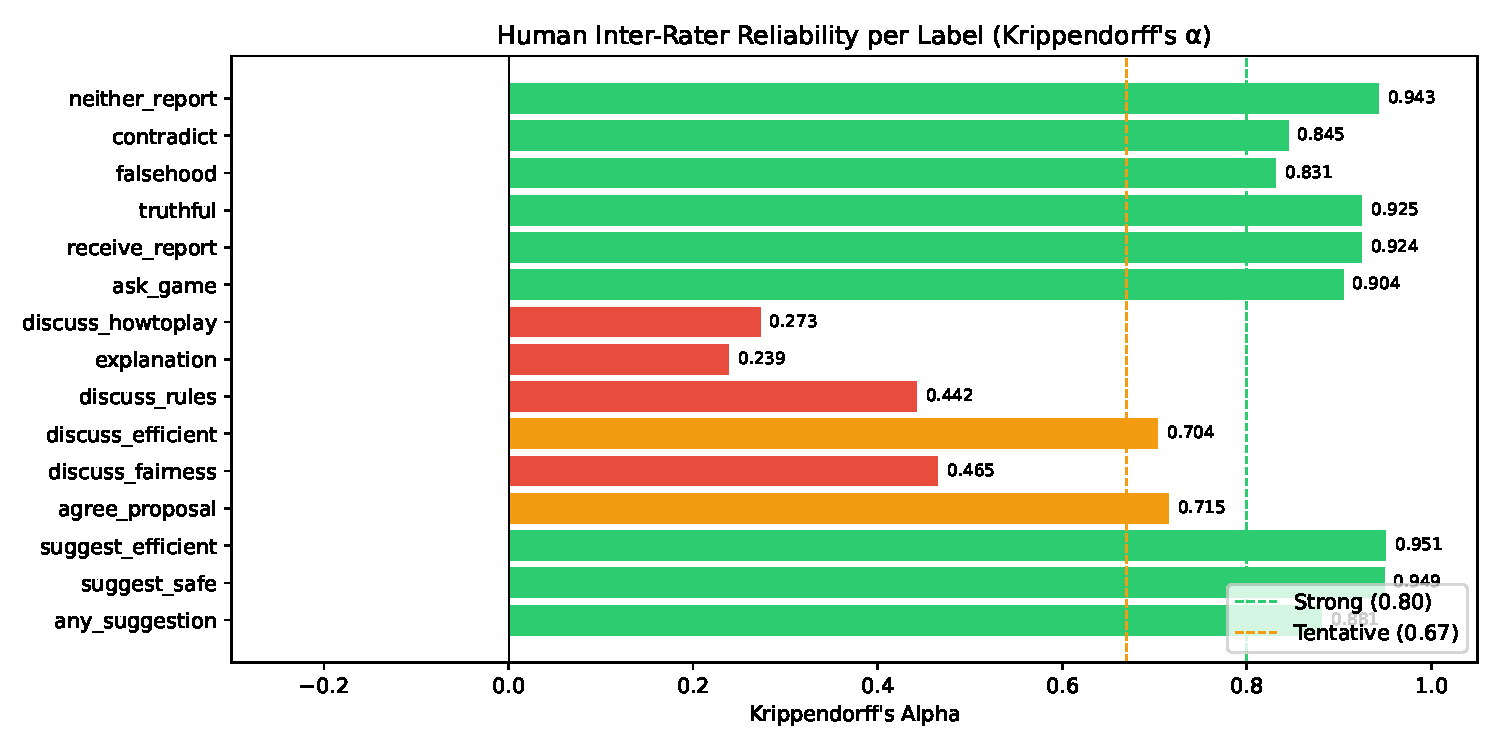
\includegraphics[width=0.9\textwidth]{1_Figures/krippendorff_alpha_plot.pdf}
\end{figure}

Figure \ref{fig:alpha_Jordi} shows that the evaluable categories fall into two broad groups. Eight are \textit{behaviorally concrete}: they capture whether agents make or agree to specific proposals, ask about the game state, or truthfully report private information, and human coders exhibit high agreement on these categories ($\alpha \geq 0.70$). The remaining four are \textit{interpretively ambiguous}: they concern broader conversational themes—such as fairness, efficiency, or rules—or require inference about communicative intent (\textit{explanation}), resulting in substantially lower human agreement ($\alpha$ ranging from 0.24 to 0.47). This distinction is important because LLMs cannot reasonably be expected to systematically exceed human inter-rater reliability; the category-specific human $\alpha$ therefore provides the relevant benchmark ceiling, rather than a uniform threshold such as 0.80.

Then, for each evaluable tag, we select the best-performing configuration for each model across all combinations of prompting strategy (zero-shot vs.\ few-shot) and temperature, and report the resulting Krippendorff's $\alpha$ as the tag-level agreement estimate. Figure \ref{fig:dot_Jordi} presents the results of this metric, treating each LLM as a fourth coder and recalculating the agreement $\alpha$. The figure plots one point for each model (Claude and GPT), representing the maximum $\alpha$ achieved across all shot-by-temperature combinations. Grey bars indicate human inter-rater agreement among the three original coders; the dashed vertical line marks $\alpha = 0.80$, which is the standard threshold in the literature for agreement among classifiers.

\begin{figure}[htbp]
\centering
    \caption{Best-configuration Krippendorff's $\alpha$ per category - \citet{brandts_cooper_2025}} \label{fig:dot_Jordi}    
    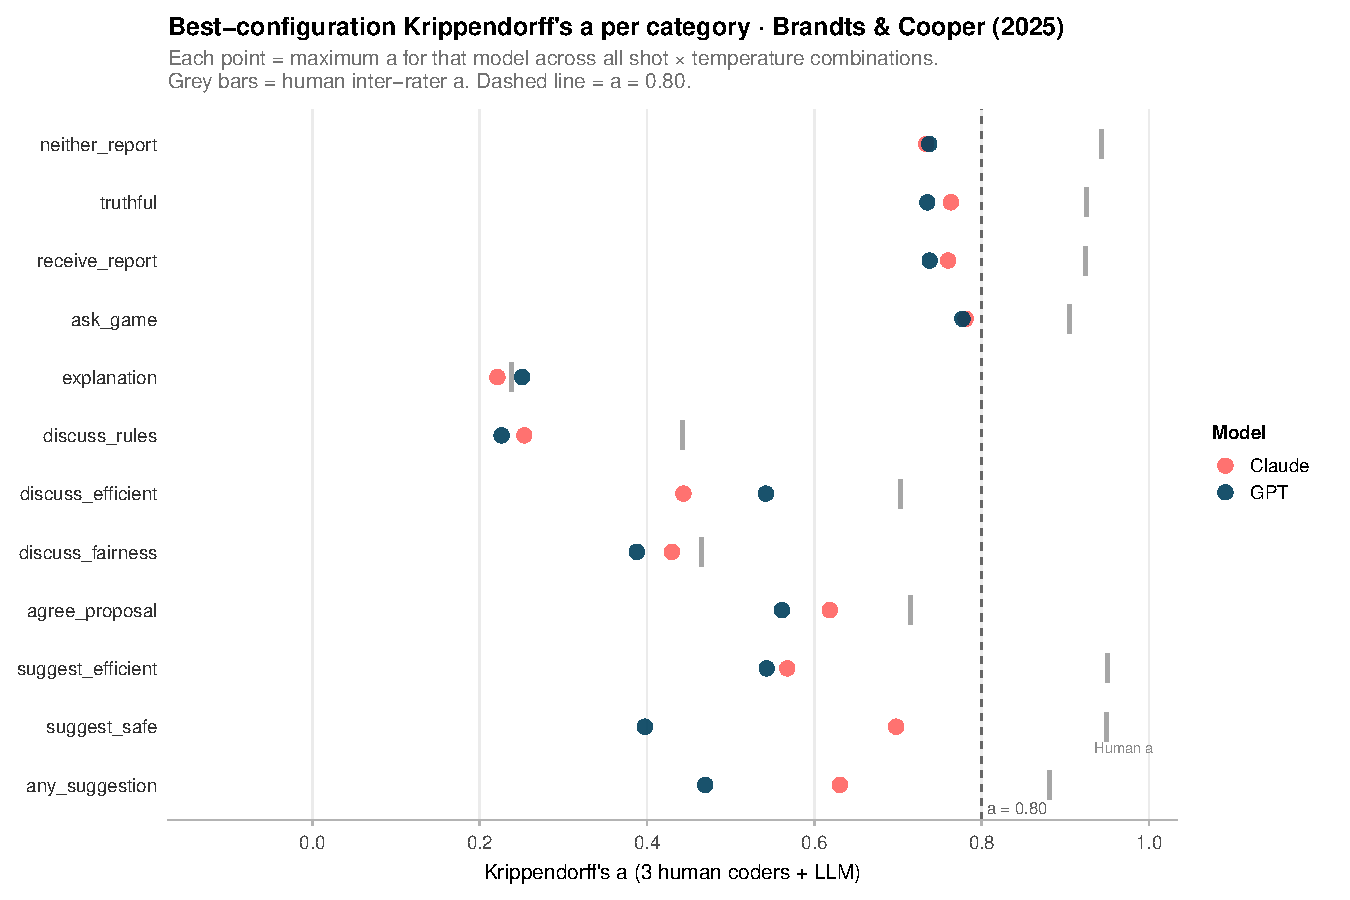
\includegraphics[width=0.9\textwidth]{1_Figures/dotplot_best_config_managerial_leadership_Jordi_Cooper.pdf}

        \footnotesize
    \textit{Note:} Each point $=$ maximum a for that model across all shot $ \times$ temperature combinations. Grey bars $=$ human inter-rater $\alpha$. Dashed line $=$ $\alpha = 0.80$.
\end{figure}


Among the 12 evaluable tags, agreement with human coders varies substantially across models. CLaude achieves the highest best-configuration $\alpha$ for seven tags. The two LLMs perform poorly on \texttt{discuss\_rules} and \texttt{discuss\_fairness}. Human agreement is also modest for these two tags, suggesting that these categories are inherently ambiguous rather than uniquely difficult for LLMs to classify. Figure \ref{fig:overall_agree_jordi} reports the average Krippendorff’s $\alpha$ across the 12 evaluable tags for each model, with configurations defined by prompting strategy (zero-shot versus few-shot) and temperature ($T \in {0, 0.1, 0.5, 1, 1.2}$). Both models achieve their strongest performance under few-shot prompting at $T = 0$, with Claude attaining the higher mean $\alpha$ across categories. Variation across temperature settings within a given prompting strategy is modest, suggesting that performance in this task is relatively insensitive to LLM's temperature.

\begin{figure}[htbp]
    \caption{Overall agreement with Human Annotations - \citet{brandts_cooper_2025}} \label{fig:overall_agree_jordi}
    \centering
    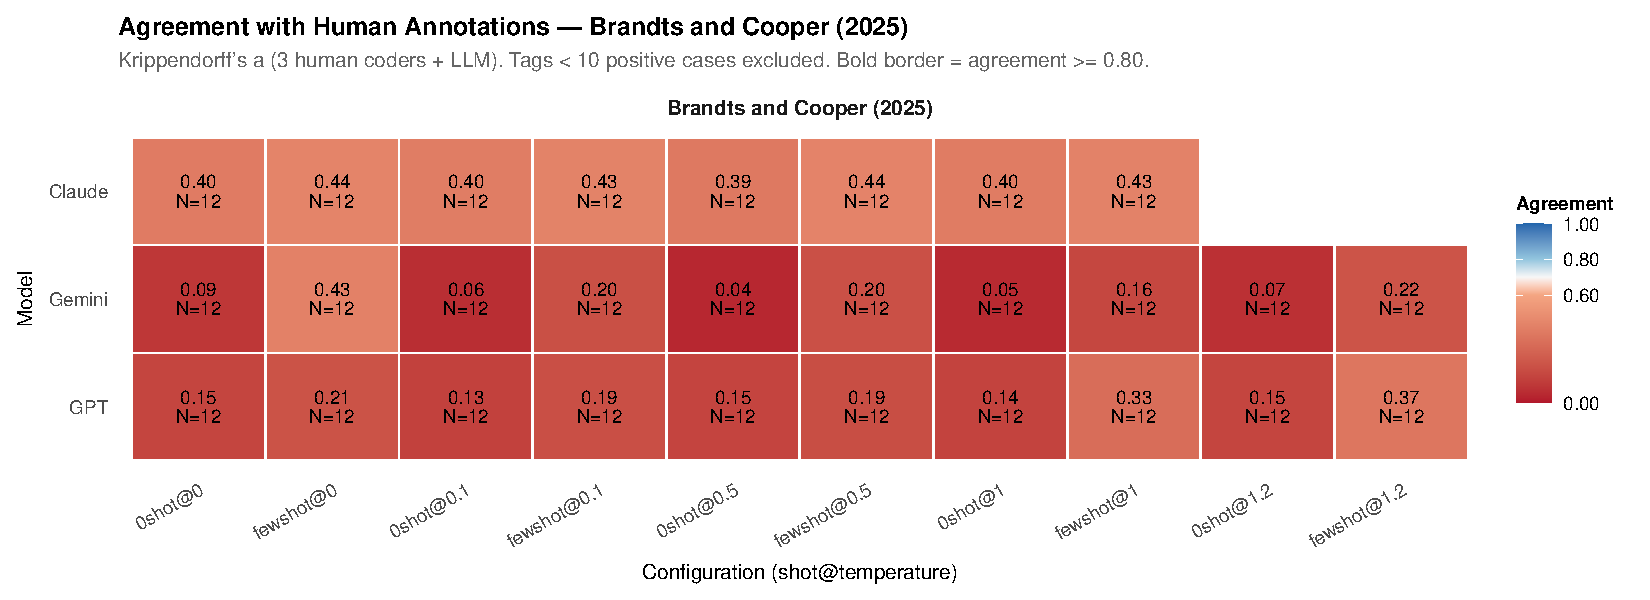
\includegraphics[width=0.9\textwidth]{1_Figures/figure1_agreement_heatmap_managerial_leadership_Jordi_Cooper.pdf}

        \footnotesize
    \textit{Note:} Krippendorff’s $\alpha$ (3 human coders + LLM). Tags $<$ 10 positive cases excluded.
\end{figure}

% \begin{figure}[htbp]
%     \caption{Temperature sensitivity of aggregate score by model and prompt style - \citet{brandts_cooper_2025}} 
%     \label{fig:figure2_temperature_Jordi}
%     \centering
%     
\includegraphics[width=0.9\textwidth]{1_Figures/figure2_temperature_sensitivity_managerial_leadership_Jordi_Cooper.pdf}
%     
%     \vspace{0.3cm}
%     \footnotesize
%     \textit{Note:} The figure displays aggregate performance across temperature values for each model (Claude, Gemini, GPT) and prompt style (0-shot and few-shot). Aggregate score corresponds to the mean across selected core metrics. 
% \end{figure}

In this paper we found that LLMs are not particularly good trying to replace humans coders. The main issue for this data is its complexity given that they used chats between three people with a lot of jargon, and implicit meaning difficult to catch. Even for humans, there were some categories were agreement was particularly low. In other words, the categories in this paper are likely interpretively ambiguous. For instance, things like "suggest safe", "discuss fairness", "agree proposal" require inferring intent or pragmatic meaning from text, which is harder than detecting more concrete or surface-level features. The LLM and the human coder are essentially applying different implicit criteria.

To assess the consistency of response classifications across temperature settings, we treat each temperature run as an independent rater and compute Krippendorff’s alpha over the resulting label vectors. This internal consistency analysis abstracts from agreement with the human benchmark and instead evaluates whether a model’s coding decisions remain stable across temperature variations. High alpha values indicate that the model produces consistent classifications regardless of temperature, whereas low values suggest that temperature meaningfully affects classification outcomes for a given category. Table \ref{tab:temp_irr_managerial} reports label-level alpha values for Claude (temperatures 0, 0.1, 0.5, and 1) and GPT (temperatures 0, 0.1, 0.5, 1, and 1.2) under both zero-shot and few-shot prompting conditions.

\input{2_Tables/irr_llms_jordi}

Table \ref{tab:temp_irr_managerial} shows that Claude achieves strong internal consistency across most categories, with mean $\alpha = 0.853$ under zero-shot prompting and $\alpha = 0.881$ under few-shot prompting. Under zero-shot prompting, only \textit{safe suggestion} falls below the 0.67 reliability threshold, while four categories fall within the tentative agreement range. Few-shot prompting reduces the number of tentative categories to two: \textit{discuss rules} and \textit{contradiction}. Conversely, GPT exhibits substantially lower internal consistency (mean $\alpha = 0.650$ under zero-shot prompting and $\alpha = 0.660$ under few-shot prompting), with four categories falling below 0.67 in the zero-shot setting. Few-shot prompting does not consistently improve GPT’s stability. These results indicate that Claude’s classifications are largely insensitive to temperature variation, whereas GPT’s coding decisions, particularly for categories requiring pragmatic inference about conversational context, vary considerably across temperature settings.


\subsubsection{\citet{brandts_cooper_2025}: substantive validity}

To evaluate substantive validity, that is, whether LLM-coded data lead to the same conclusions as human-coded data, we link both human- and LLM-generated labels to the replication outcomes at the conversation-round level and restrict attention to the free-chat treatments. This analysis relies on files provided by the authors through their replication package and subsequent correspondence. The shared chat files do not include CH/A-D sessions, although the coding file contains CH/A-D observations for which no corresponding message-level source data are available. Because these source data are absent from the shared materials, the corresponding observations cannot be classified by the LLMs. Accordingly, all LLM-based analyses are restricted to the treatments covered by the shared files, and results requiring CH/A-D observations fall outside the scope of this analysis. For all analyses, we use the few-shot prompting configuration at temperature $T = 0$.

We then replicate the core regression analysis of \citet{brandts_cooper_2025}, which examines how communication content predicts coordination outcomes. Table 8 in the original paper reports Probit regressions in which binary coordination outcomes, whether a group coordinated, and whether coordination was
efficient, are regressed on the chat content categories, separately by treatment. We replicate this specification as a Probit model on the restricted shared-data sample, replacing the human-coded categories with LLM-generated categories in turn, so that all columns (human, Claude, GPT, ensemble) are estimated on the same observations.

Table \ref{tab:table8-lpm-condensed} reports results across three panels: coordination in CH/S-D, efficient coordination in CH/S-D, and efficient coordination in CH-MC. In the \textit{CH/S-D coordination} panel, the human-coded benchmark indicates a positive and statistically significant effect of \textit{Agreement} ($\beta = 0.196$, $p < 0.01$), broadly consistent with the original benchmark estimate ($\beta = 0.108$). GPT-based coding also yields a positive and marginally significant effect for \textit{Agreement} ($\beta = 0.057$, $p < 0.10$). By contrast, Claude-based coding produces a positive and statistically significant effect for \textit{Questions about play} ($\beta = 0.050$, $p < 0.01$), a relationship that does not appear in the human-coded benchmark.

In the \textit{CH/S-D efficient coordination} panel, the human-coded benchmark remains broadly consistent with the pattern reported in the original paper. Claude-based coding yields positive and statistically significant effects for \textit{Discuss need to coordinate}, \textit{Discuss fairness}, and \textit{Discuss efficiency}, whereas GPT-based coding does not produce statistically significant effects in this specification.

Finally, in the \textit{CH-MC efficient coordination} panel, the human-coded benchmark again closely matches the replication-package estimate for \textit{Truthfully reveal game} ($\beta = 0.290$, $p < 0.01$; paper estimate: $0.295$). GPT-based coding produces a negative and statistically significant effect for \textit{Explanation} ($\beta = -0.171$, $p < 0.05$) and a positive and statistically significant effect for \textit{Lie about game} ($\beta = 0.432$, $p < 0.01$). The ensemble specification also yields a positive and statistically significant effect for \textit{Lie about game} ($\beta = 0.261$, $p < 0.05$).

Overall, the Probit regressions lead to the same qualitative conclusion: LLM-derived codings do not consistently reproduce the human-coded benchmark coefficients in this application. Some alignment emerges for selected variables—for example, the positive association between \textit{Agreement} and CH/S-D coordination in the GPT-based specification—but several statistically significant LLM-derived coefficients differ from the human benchmark in either sign or substantive prominence. This pattern is consistent with the agreement analysis discussed above: categories characterized by greater interpretive ambiguity tend to produce less stable downstream substantive inferences.


\input{2_Tables/table8_replication}

 
\subsection{Application 2: Messages and promises in a trust game over time 
\citep{ederer_schneider_2022}}

The second application we consider is \citet{ederer_schneider_2022}. The authors examine how temporal delay affects trust, trustworthiness, and the credibility of promises, motivated by the empirical observation that trust often involves delayed reciprocation. Using a large-scale hybrid laboratory–online experiment with over 700 participants, they employ an adaptation of the trust game \citep{berg1995trust, guth1997cooperation}, similar to that proposed by \citet{charness2006promises}, by introducing exogenous time delays between the trustor's decision to send money and the trustee's opportunity to reciprocate. The experimental design varies three temporal conditions: immediate decisions during the laboratory session, early decisions within 24 hours, and late decisions after a 21-day delay. Crucially for our purposes, they incorporate a pre-play communication stage that allows trustees to send free-form messages, including non-binding promises, to trustors. This design allows for an examination of whether the positive effects of communication on cooperative behavior persist when reciprocation is delayed, testing the hypothesis that temporal distance may erode both the propensity to honor commitments and the overall level of trustworthiness.

The experiment measures trust by the amount sent by trustors and trustworthiness by the amount returned by trustees, with trustees making 10 binary ROLL/DON’T ROLL choices, one of which is randomly implemented. To analyze free-form communication, the authors employ two hypothesis-blind research assistants to independently classify messages according to whether they contain an explicit promise to choose ROLL (e.g., “I will choose ROLL” or “I promise to choose ROLL”). \citet{ederer_schneider_2022} find that pre-play communication substantially increases cooperation, trust, and trustworthiness by approximately 50 percent, with this effect remaining robust even when three weeks elapse between the trustee's message and their actual reciprocation decision. Across all three delay conditions (Immediate, Early, and Late), the passage of time does not significantly affect trust or trustworthiness, suggesting that findings from standard laboratory settings generalize to environments with greater external validity. Trustees who make promises exhibit higher ROLL rates (6.2 choices on average) compared to those who do not (4.2 choices), while trustors increase their IN choices by approximately 20 percentage points when communication is possible, with both effects remaining consistent across time frames. Analysis of the free-form chat data confirms that explicit promises are the primary driver of these effects.


\subsubsection{\citet{ederer_schneider_2022}: validation metrics}

In the first application, we used Claude and GPT as the evaluated LLMs. In the subsequent two applications, we additionally included Gemini. Gemini is substantially more expensive, costing approximately two to three times more than Claude and up to five times more than GPT. Because the first application involved a more computationally demanding dataset, we restricted the use of Gemini to the second and third applications.

For this paper, we do not report Krippendorff’s alpha because only one human classification is available for each tag. Accordingly, we focus on Cohen’s kappa as the primary agreement metric. Figure \ref{fig:dot_ederer} presents the Cohen’s kappa values for the three analyzed categories. As in Application 1, we select the best-performing configuration for each model across all combinations of prompting strategy (zero-shot versus few-shot) and temperature, and report the resulting Cohen’s kappa as the tag-level agreement estimate. The figure displays one point for each model (Claude, Gemini, and GPT), corresponding to the maximum $\kappa$ achieved across all shot-by-temperature combinations. The dashed vertical line marks $\kappa = 0.80$, the conventional threshold in the literature for strong agreement among classifiers.


\begin{figure}[htbp]
\centering
    \caption{Best-configuration Cohen's $\kappa$ per category - \citet{ederer_schneider_2022}} \label{fig:dot_ederer}    
    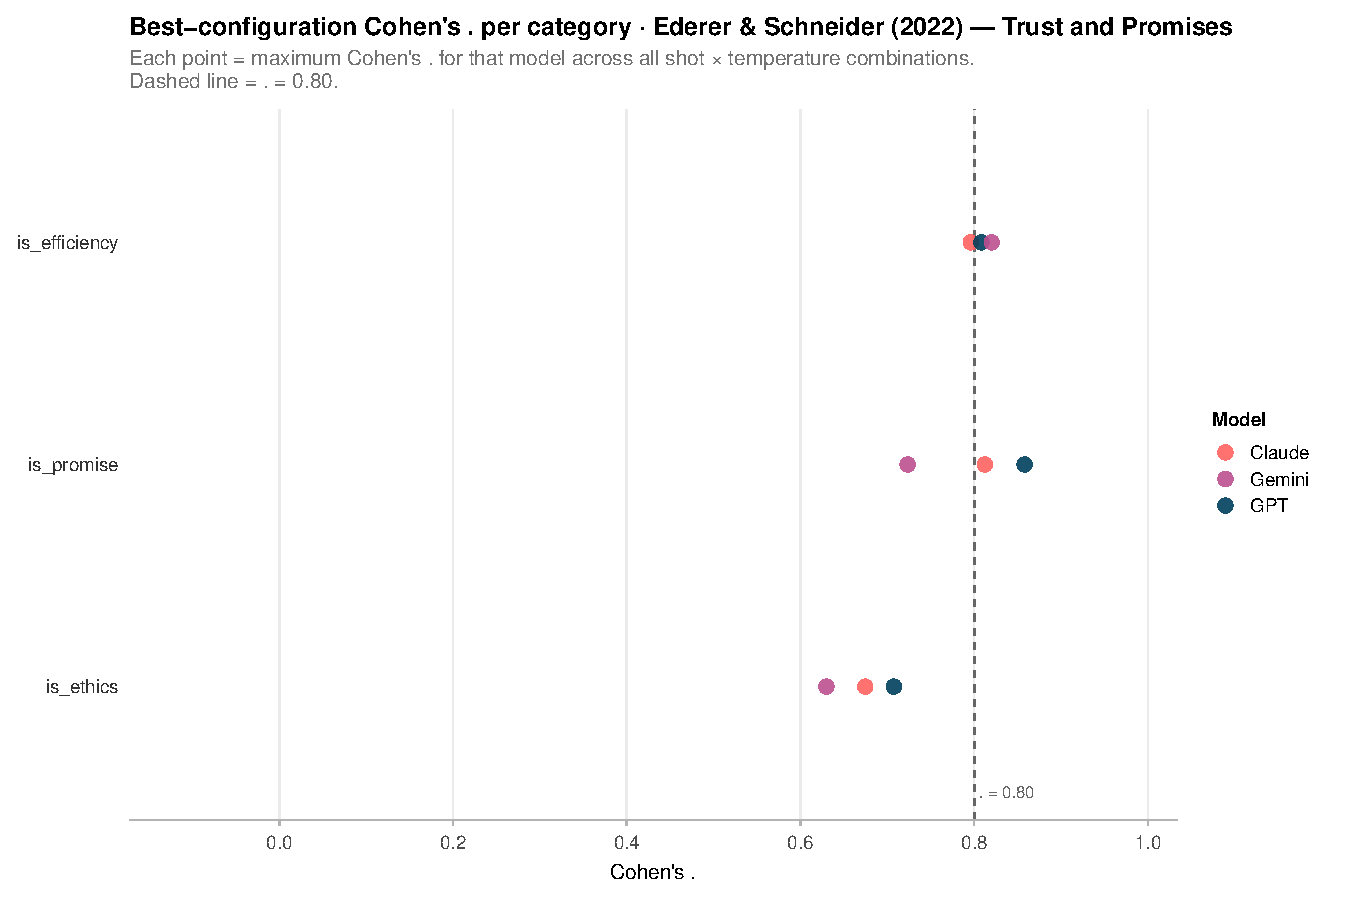
\includegraphics[width=0.9\textwidth]{1_Figures/dotplot_best_config_trust_promises_Ederer_Schneider.pdf}

        \footnotesize
    \textit{Note:} Each point $=$ maximum a for that model across all shot $ \times$ temperature combinations. Grey bars $=$ human inter-rater $\kappa$. Dashed line $=$ $\kappa= 0.80$.
\end{figure}

Figure~\ref{fig:dot_ederer} shows that the categories \texttt{is\_promise} and \texttt{is\_efficiency} achieve high agreement between LLMs and human coders, with the exception of Gemini on \texttt{is\_promise}. In contrast, the category \texttt{is\_ethics} exhibits lower Cohen’s kappa values across models.

Overall, the categories in this application correspond to relatively well-defined normative concepts that language models can identify from the surface and semantic features of the text. Unlike Application 1, classification in this setting does not require tracking conversational context or inferring pragmatic intent. Moreover, the dataset does not suffer from severe class imbalance, meaning that each category contains a sufficient number of positive cases to support meaningful agreement estimates.

The comparatively lower agreement for \texttt{is\_ethics} may indicate that LLMs tend to over-predict ethical content, labeling statements as ethical when the human coder did not. As a result, the mean agreement values reported in Figure~\ref{fig:overall_agree_ederer} fall below the 0.80 threshold, with the lower performance of this category reducing overall agreement levels. This asymmetry is noteworthy because ethics is likely the most interpretation-dependent of the three categories.

\begin{figure}[htbp]
    \caption{Overall agreement with Human Annotations - \citet{ederer_schneider_2022}} \label{fig:overall_agree_ederer}
    \centering
    
\includegraphics[width=0.9\textwidth]{1_Figures/figure1_agreement_heatmap_trust_promises_Ederer_Schneider.pdf}

        \footnotesize
    \textit{Note:} Cohen’s $\kappa$ (human coder + LLM).
\end{figure}

Finally, Table \ref{tab:temp_irr_trust} reports internal consistency across temperature settings for the trust-promises application. All model-strategy combinations achieve strong Krippendorff's alpha values, with no entry falling below the 0.80 threshold. Claude is the most consistent model, attaining near-perfect agreement under zero-shot prompting (mean $\alpha = 0.994$), with \textit{promise} and \textit{ethics} reaching 1.000 and \textit{efficiency} reaching 0.982. Few-shot prompting yields similarly high stability (mean $\alpha = 0.979$). Gemini is likewise highly consistent, with mean alpha values of 0.902 under zero-shot prompting and 0.918 under few-shot prompting, although the \textit{ethics} category is somewhat less stable (0.845 under zero-shot prompting and 0.870 under few-shot prompting). We can also see in Figure \ref{fig:overall_agree_ederer} that Gemini was the worse performing LLM.

The near-ceiling consistency observed across all model-strategy combinations likely reflects the conceptual clarity of the three coding categories. A message either contains an explicit promise, an efficiency argument, or an ethical argument, each of which can be identified from surface-level semantic features of the text without requiring substantial inference about conversational context or pragmatic intent. Overall, this application provides the clearest example of the conditions under which LLM-based coding performs well: a small number of well-defined, non-overlapping categories with balanced class representation.

\begin{table}
    \centering
    \caption{Internal consistency across temperature settings -- \citet{ederer_schneider_2022}}
    \label{tab:temp_irr_trust}
    \begin{adjustbox}{max width=0.95\linewidth}
    \small
    \begin{tabular}{lcccccc}
        \toprule
        & \multicolumn{2}{c}{Claude} & \multicolumn{2}{c}{GPT} & \multicolumn{2}{c}{Gemini} \\
        \cmidrule(lr){2-3}\cmidrule(lr){4-5}\cmidrule(lr){6-7}
        Category   & Zero-shot & Few-shot & Zero-shot & Few-shot & Zero-shot & Few-shot \\
        \midrule
        Promise    & 1.000 & 0.990 & 0.978 & 0.969 & 0.900 & 0.980 \\
        Efficiency & 0.982 & 0.983 & 0.984 & 0.957 & 0.962 & 0.902 \\
        Ethics     & 1.000 & 0.965 & 0.900 & 0.904 & 0.845 & 0.870 \\
        \midrule
        \textit{Mean} & \textit{0.994} & \textit{0.979} & \textit{0.954} & \textit{0.943} & \textit{0.902} & \textit{0.918} \\
        \bottomrule
    \end{tabular}
    \end{adjustbox}
    \vspace{0.2cm}
    \begin{minipage}{0.95\linewidth}
        \footnotesize
        \textit{Note:} Krippendorff's alpha treating each temperature run as an independent rater (predictions binarized: ${>}0.5\to 1$, else~0). Claude: 4 temperature settings (0, 0.1, 0.5, 1). GPT and Gemini: 5 settings (0, 0.1, 0.5, 1, 1.2). All values indicate strong agreement ($\alpha\geq0.80$).
    \end{minipage}
\end{table}


\subsubsection{\citet{ederer_schneider_2022}: substantive validity}

To assess whether the same substantive conclusions emerge when using LLM-coded data instead of human-coded data, we use the replication package provided by the authors on the publication website. Among the three coded labels, only \textit{is\_promise} is used in the published analysis of \citet{ederer_schneider_2022}. The authors code whether each trustee message contains an explicit promise to choose ROLL and use this classification in a single core regression: an \textsc{OLS} specification of \textit{numrolls} (the number of ROLL choices out of 10) on a communication-treatment indicator and \textit{is\_promise}, restricted to trustees (\textit{role} $= 1$, $N = 354$), with standard errors clustered at the session level. In the original paper, this specification yields a positive and statistically significant effect for \textit{is\_promise}, indicating that trustees who explicitly promise to cooperate choose ROLL substantially more often than those who do not.

To address this question, we replace the human-coded \textit{is\_promise} variable with LLM-generated predictions from each model using the zero-shot, temperature-$0$ configuration, which achieved the strongest agreement performance for this label in the analysis above. For trustees in the no-communication condition, \textit{is\_promise} is set equal to 0 for all models, consistent with the original coding procedure, as these participants did not send a message and therefore could not make a promise. For the 172 trustees who sent messages, LLM predictions are merged using the message text as the matching key. The regression specification is otherwise identical to that used in the original paper.

Table \ref{tab:ederer_regression} reports the results. The human-coded baseline closely reproduces the original finding ($\hat{\beta} = 1.977$, $p = 0.037$).\footnote{These results may differ slightly from those reported in the original paper because some observations are lost during the classification process; accordingly, we restrict the analysis to the subset of observations also coded by the LLMs.} Under LLM-based coding, the coefficient on \textit{Promise} retains the same sign and a broadly similar magnitude across all three models, although statistical significance weakens. GPT comes closest to reproducing the original result ($\hat{\beta} = 1.746$, $p = 0.060$), while Gemini ($p = 0.085$) and Claude ($p = 0.128$) fall further from conventional significance thresholds. The communication-treatment indicator is not statistically significant in any specification, consistent with the original paper.

\input{2_Tables/table_p2_sustantive}

Overall, these results suggest that when the classification task is relatively straightforward, LLM-based coding can recover the same qualitative substantive conclusions as human coding. Although the LLM-based estimates exhibit greater noise, leading in some cases to weaker statistical significance, the direction and approximate magnitude of the effects remain broadly consistent with the human-coded benchmark.

The remaining two labels, \textit{is\_efficiency} and \textit{is\_ethics}, appear only in the appendices as descriptive statistics. Efficiency appeals are present in 49 per cent of messages and are strongly correlated with promise-making ($r = 0.75$), whereas ethics appeals appear in only 8 per cent of messages.

Table \ref{tab:ederer_descriptives} extends the comparison to the secondary labels reported descriptively in Appendix D of \citet{ederer_schneider_2022}. Panel A reports prevalence rates among the 172 trustees in the communication condition. For \textit{Promise}, Claude and GPT produce estimates close to the human benchmark (67.4\% versus 69.8\%), whereas Gemini overpredicts the category (79.1\%). For \textit{Efficiency}, all three models substantially overpredict relative to the human coder (57-59\% versus 49\%), suggesting that LLMs identify efficiency-related language more broadly than the comparatively conservative human coding standard. The divergence is largest for \textit{Ethics}: the human coder identifies ethics appeals in only 7.6\% of messages, compared with 12.2\% for Claude, 9.9\% for GPT, and 22.1\% for Gemini. This pattern is consistent with a tendency for LLMs to classify implicit normative language as ethical framing even when a human coder would not interpret it as an explicit ethics appeal.

Panel B reports Pearson correlations for the full trustee sample ($N = 354$). The correlation between \textit{Promise} and \textit{Efficiency} is closely reproduced by Claude ($r = 0.699$ versus the human benchmark of $0.709$) and reasonably approximated by GPT ($r = 0.671$), while Gemini produces a somewhat higher estimate ($r = 0.774$). By contrast, the correlation between \textit{Promise} and \textit{Ethics} is more distorted. The human benchmark of $r = 0.146$ increases to $0.181$ under Claude, $0.237$ under GPT, and $0.383$ under Gemini, reflecting the tendency of the models, particularly Gemini, to overpredict ethics-related labels and thereby inflate apparent co-occurrence.

\input{2_Tables/tab_ederer_descriptive_sustantive}


\subsection{Application 3: Social Desariability Bias and AI use \citep{ling2025underreporting} }

The third application draws on data from \citet{ling2025underreporting}, in which the authors study the discrepancy between self-reported AI usage and perceived peer usage in educational settings. The authors attribute this gap primarily to social desirability bias \citep{krumpal2013determinants}. The study employs an indirect questioning method, commonly used in the psychology literature \citep{fisher1993social}, with 338 university students, by asking respondents to report both their own AI use and their perceptions of peers’ usage. Results reveal that approximately 60\% of students report using AI themselves, compared to nearly 90\% when reporting on peer usage. Qualitative evidence indicates that a majority of students (70.8\%) attribute this gap to reluctance to admit their own use of large language models, a pattern consistent with the documented social norm of “AI shaming” across academic and professional settings. Additional mechanisms contributing to this gap include overestimation of peers’ usage driven by availability bias and information asymmetry regarding actual adoption rates.

To investigate the mechanisms underlying this discrepancy, the researchers collected open-ended responses from a separate follow-up survey involving 96 undergraduate students recruited via Prolific. This sample serves as the benchmark for our analysis. Participants were presented with findings from the initial survey, highlighting the reporting gap, and asked an open-ended question to explain it in their own words. These responses were analyzed using a streamlined thematic analysis approach: the first author conducted open coding to identify proposed explanations, after which all authors jointly refined and agreed upon a set of inductive codes, which were then iteratively applied to classify each response, with ambiguous cases resolved through author consultation. This coding process identifies social desirability bias as the most frequently cited explanation for the reporting gap, while also surfacing alternative mechanisms such as overestimation of peers' AI usage driven by availability bias and information asymmetry regarding actual adoption rates among peers. This application is particularly well-suited for evaluating whether LLMs can reproduce inductive thematic coding on short explanatory responses. The findings demonstrate that self-reported AI adoption statistics are substantially distorted by social desirability bias and that indirect questioning, by making individuals more comfortable attributing sensitive behaviors to peers, provides a more accurate measure of underlying AI adoption, with important implications for institutional policy, stigma reduction, and responsible AI integration strategies.


\subsubsection{\citet{ling2025underreporting}: validation metrics}

For this application we also use Cohen’s kappa as the primary agreement metric. The coding categories used by \citet{ling2025underreporting} captures twelve distinct mechanisms that may explain the gap between personal and peer-reported AI usage. \textit{Uninformative} responses contain nonsensical or contradictory content that misunderstands the question. \textit{SDB} (Social Desirability Bias) refers to the possibility that individuals misreport or conceal AI usage to avoid negative social evaluation, judgment, or reputational harm. \textit{Academic\_integrity} captures concerns that AI usage constitutes cheating, dishonesty, or academically inappropriate behavior. \textit{Overest\_others} indicates that students overestimate their peers’ AI usage, whereas \textit{Underest\_own} reflects students underestimating their own usage. \textit{Info\_asymmetry} captures students’ limited knowledge about their peers’ actual AI usage patterns. \textit{Privacy\_concerns} reflects reluctance to disclose personal AI usage because of privacy considerations. \textit{Self\_esteem} indicates that students underreport usage to protect their internal self-image, distinct from concerns about external judgment captured by \textit{SDB}. \textit{Self\_report\_bias} captures broader self-enhancement or self-favoring biases in reported behavior.
\textit{AI\_discussion\_priming} attributes the gap to confusion between the visibility and frequency of AI-related discussions or media coverage and the actual prevalence of AI usage. \textit{Network\_effect} explains the gap by suggesting that students generalize from their local social networks, inferring broader population-level AI usage from the behavior observed within their immediate peer group. Finally, \textit{Truthful} indicates that the reported gap reflects genuine differences between personal and peer AI usage.

Figure \ref{fig:dot_liang} presents the Cohen’s kappa values for the twelve coding categories. As in the previous applications, we select the best-performing configuration for each model across all combinations of prompting strategy (zero-shot versus few-shot) and temperature, and report the resulting Cohen’s kappa as the tag-level agreement estimate. The figure displays one point for each model (Claude, Gemini, and GPT), corresponding to the maximum $\kappa$ achieved across all shot-by-temperature combinations. The dashed vertical line marks $\kappa = 0.80$, the conventional threshold for strong agreement.

\begin{figure}[htbp]
\centering
    \caption{Best-configuration Cohen's $\kappa$ per category - \citet{ling2025underreporting}} \label{fig:dot_liang}    
    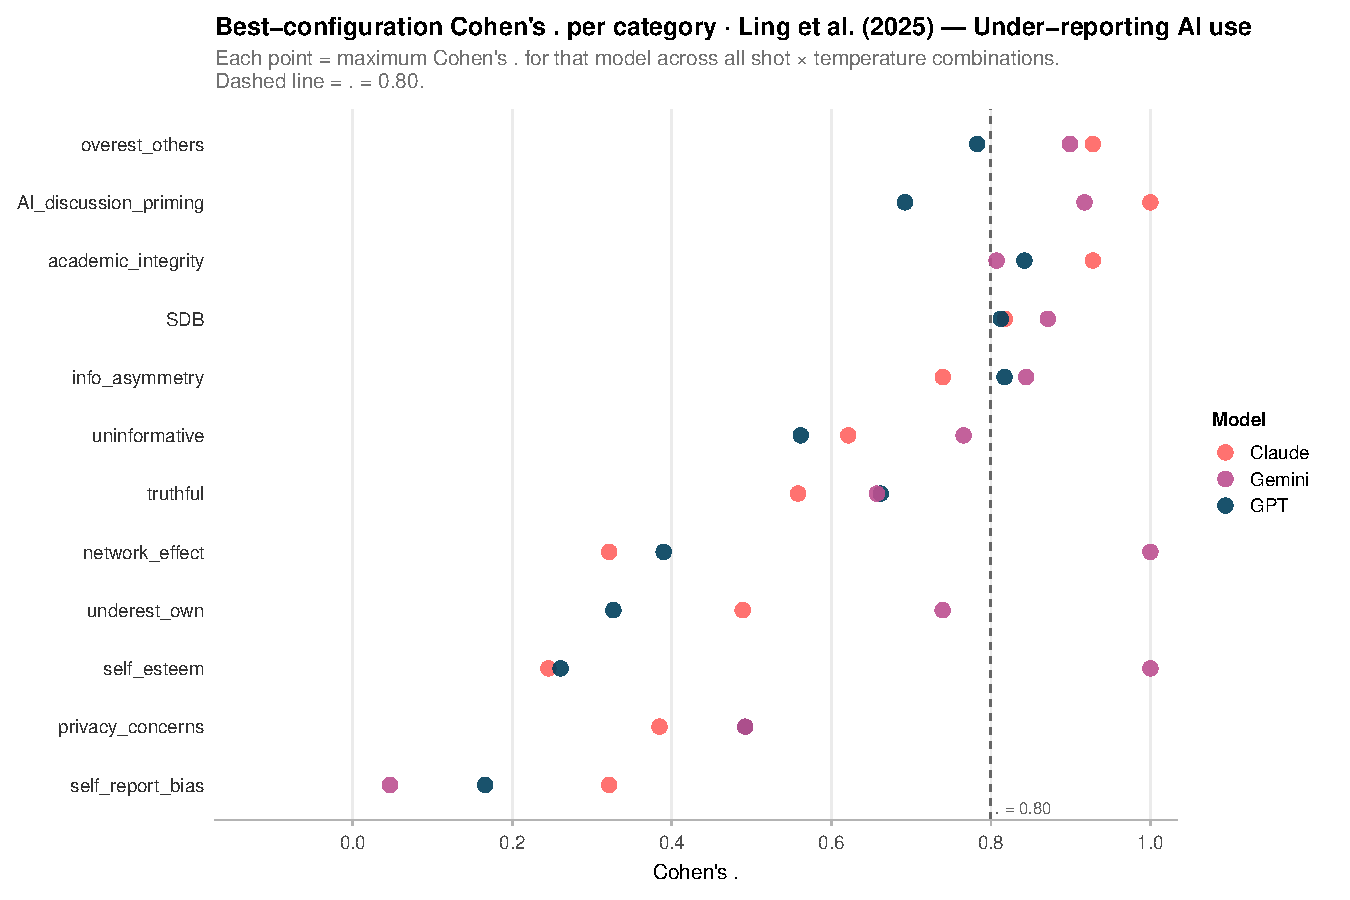
\includegraphics[width=0.9\textwidth]{1_Figures/dotplot_best_config_under_reporting_Ling_Kale_Imas.pdf}

        \footnotesize
    \textit{Note:} Each point $=$ maximum a for that model across all shot $ \times$ temperature combinations. Grey bars $=$ human inter-rater $\kappa$. Dashed line $=$ $\kappa= 0.80$.
\end{figure}


Figure \ref{fig:dot_liang} shows substantial heterogeneity in agreement across categories. Four categories---\textit{overestimate peers}, \textit{social desirability bias}, \textit{academic integrity}, and \textit{information asymmetry}---reach or closely approach the $\kappa = 0.80$ threshold for strong agreement between the human coding and each LLM. This pattern is consistent with the explicit theoretical grounding of these constructs and the relative clarity with which they are expressed in respondents’ answers.

In contrast, \textit{self-report bias}, \textit{network effect}, and \textit{privacy concerns} remain well below the threshold for every model, even under the best-performing configuration. This likely reflects both the more inductive origins of these labels and the inferential demands they place on coders, who must attribute implicit motivations to short, open-ended responses.

A notable outlier is the \textit{self-esteem} category, for which Gemini achieves near-perfect agreement ($\kappa \approx 1.0$), whereas Claude and GPT both fall below $0.25$. Such extreme divergence is more plausibly attributable to Gemini collapsing class variation by systematically predicting a single value than to genuine alignment with human judgment. Class-balance diagnostics should therefore be examined before interpreting this result as evidence of superior performance.

Figure \ref{fig:overall_agree_liang} presents Cohen’s $\kappa$ relative to the human benchmark across all ten shot $\times$ temperature configurations for the five categories meeting the minimum prevalence threshold. Gemini achieves the highest and most stable agreement, with $\kappa$ values ranging narrowly from 0.73 to 0.78 and showing minimal sensitivity to prompting strategy or temperature. Claude performs similarly under zero-shot prompting ($\kappa = 0.70$--$0.73$) but deteriorates under few-shot prompting at lower temperatures, suggesting that the examples may introduce an interfering prior. GPT exhibits the greatest variability, with $\kappa$ ranging from 0.39 to 0.74, although few-shot prompting generally improves performance relative to zero-shot. Overall, even the best-performing configurations achieve only moderate agreement, reflecting the inductive nature of the coding scheme for some categories, which requires inference about social motivations rather than identification of surface-level linguistic features.

\begin{figure}[htbp]
    \caption{Overall agreement with Human Annotations - \citet{ling2025underreporting}} \label{fig:overall_agree_liang}
    \centering
    
\includegraphics[width=0.9\textwidth]{1_Figures/figure1_agreement_heatmap_under_reporting_Ling_Kale_Imas.pdf}

        \footnotesize
    \textit{Note:} Cohen’s $\kappa$ (human coder + LLM).
\end{figure}

Table \ref{tab:temp_irr_under} reports internal consistency across temperature settings for the under-reporting application. All three models achieve strong mean alpha values, although notable variation emerges for specific labels. Claude attains the highest and most uniform consistency, with mean $\alpha = 0.950$ under zero-shot prompting and $\alpha = 0.973$ under few-shot prompting; three labels exhibit no cross-temperature variance in a given strategy (shown as ---) and are therefore excluded from the mean calculation. Gemini is also broadly consistent (mean $\alpha = 0.825$ under zero-shot prompting and $\alpha = 0.827$ under few-shot prompting), although two labels fall below the reliability threshold: \textit{underestimate self} ($\alpha = 0.621$ under zero-shot prompting) and \textit{network effect} ($\alpha = 0.527$ under zero-shot prompting; $0.604$ under few-shot prompting). GPT achieves strong mean consistency under zero-shot prompting ($\alpha = 0.885$), with only \textit{self-report bias} (0.752) and \textit{truthful response} (0.768) falling within the tentative agreement range and no category below 0.67. Notably, the problematic labels for Gemini (\textit{underestimate self} and \textit{network effect}) are among the most inductively defined categories in the coding scheme, suggesting that nuanced social-psychological constructs are more sensitive to temperature variation than more concrete thematic labels such as \textit{social desirability bias} or \textit{academic integrity}.


\input{2_Tables/iir_llms_liang}


\subsubsection{\citet{ling2025underreporting}: substantive validity}

Finally, as in the previous applications, we examine whether using LLM-coded data instead of the authors’ original classifications would lead to the same substantive conclusions. \citet{ling2025underreporting} report category prevalence estimates showing that social desirability bias (\textit{SDB}) is the dominant explanation for the own--other AI usage gap, appearing in 60.6\% of valid responses, followed by overestimation of others’ usage (29.6\%), information asymmetry (26.8\%), and academic integrity concerns (21.1\%). The key substantive validity question in this application is therefore whether LLM-based coding reproduces the rank ordering and relative magnitudes of these categories closely enough to preserve the paper’s qualitative conclusions.

Table \ref{tab:ling_prevalence} reports prevalence rates from the human coding and from each model under zero-shot prompting at temperature 0. The main conclusion of \citet{ling2025underreporting}, namely, that social desirability bias (\textit{SDB}) is the dominant mechanism underlying the own-other AI usage gap, is robustly preserved across all three models. LLM-estimated SDB prevalence ranges from 57.5\% (Claude) to 63.2\% (Gemini), closely bracketing the human benchmark of 60.6\%. Information asymmetry and academic integrity are likewise reproduced with high fidelity, with no model deviating by more than five percentage points from the human benchmark for either category. Overall, these results suggest that the paper’s central substantive conclusions--that SDB is the primary driver of underreporting, that overestimation of peers’ AI usage plays a secondary role, and that information asymmetry represents a distinct explanatory mechanism--are reliably recovered through LLM-based coding.

\input{2_Tables/table_p3_sustantive}

\section{Discussion and conclusion}\label{s-discussion}

% =========================================================================
% STRUCTURE NOTE (delete before submission):
% Five subsections: (1) Synthesis, (2) Taxonomy of coding tasks,
% (3) Agreement vs. substantive validity, (4) Practical guidance,
% (5) Limitations + Conclusion.
% [DRAFT] = ready prose. [AUTHOR: ...] = your judgment needed there.
% =========================================================================

%--- 1. SYNTHESIS -----------------------------------------------------------
\subsection*{Synthesis of findings}

This paper provides systematic evidence on whether large language models can reliably code the kinds of open-ended text data that arise in experimental economics research. Our three applications span a wide range of coding complexity---from inductively constructed thematic schemes applied to short survey responses, to multi-label conversational coding of free-form chat in strategic environments, to binary deductive labeling of promise content in a trust game---and together allow us to identify the structural features of a coding task that determine how far LLMs can be trusted as measurement instruments.

The clearest positive finding concerns coding tasks defined by explicit, deductively specified categories whose content is surface-marked in the text. In Application~2, the promise label in \citet{ederer_schneider_2022} is precisely this type: a trustee either commits to a specific action or does not, and the relevant evidence is largely visible in the syntactic surface of the message. All three models achieve strong agreement with the human benchmark, and the main substantive conclusion of the original paper---that promise-making strongly predicts cooperative behavior---is recovered by LLM coding in terms of sign and magnitude, even if statistical significance attenuates slightly. This result extends to the descriptive secondary labels, where prevalence estimates are broadly comparable to human coding, with the main discrepancy being a tendency to over-detect ethics language, consistent with LLMs' known sensitivity to normatively framed content.

The picture is more mixed in Application~3, where the coding scheme of \citet{ling2025underreporting} is inductive rather than deductive. For the dominant and theoretically central category---social desirability bias---all three models closely reproduce the human benchmark (57--63\% vs.\ 60.6\%), and the paper's first-order substantive conclusion is preserved. However, for the tail of rare, inductively derived categories, LLM coding diverges substantially and systematically: self-esteem concerns and self-report bias are massively over-detected by most models (self-esteem inflated from 4.2\% to 14--25\%), while overestimation of peers and AI discussion priming are consistently under-detected. A researcher relying on LLM coding alone for these minor categories would draw materially different conclusions about the social-psychological portrait of students' reasoning about AI use.

The most demanding application is Application~1, the multi-label conversational coding in \citet{brandts_cooper_2025}. For the eight behaviorally concrete categories, where human coders achieve strong agreement ($\alpha \geq 0.70$), LLM coding attains moderate to good agreement. For the four interpretively ambiguous categories ($\alpha < 0.50$ among human coders), LLM performance deteriorates, mirroring the difficulty that human experts face. Critically, the downstream Probit regressions do not replicate reliably under LLM coding: some coefficients change sign, others achieve significance on variables that are not significant in the human benchmark, and the correspondence is inconsistent across models. This application illustrates the most consequential failure mode: when LLMs disagree with humans on categories that are key predictors in the regression, the conclusions can be actively misleading rather than merely noisier.

% [AUTHOR: Consider adding a 2--3 sentence synthesis paragraph here that
% explicitly places the three applications on a performance gradient, e.g.:
% "Application 2 is a near-success; Application 3 a partial success at
% the category level but reliable for first-order conclusions; Application 1
% a qualified failure at the downstream inference level for the most
% complex coding categories." A crisp ranking helps readers who read
% the conclusion before the results.]

%--- 2. TAXONOMY OF CODING TASKS -------------------------------------------
\subsection*{What predicts LLM performance: a taxonomy}

Across the three applications, a consistent pattern emerges: the structural features of the coding scheme---not the choice of model or temperature---are the primary determinants of LLM coding quality. We identify three features that appear to matter most.

\textit{Deductive versus inductive scheme construction.} Categories derived from prior theory and defined before data collection tend to be more reliably coded by LLMs because they correspond to constructs whose semantic content is relatively stable and can be communicated through a prompt. Inductive categories, constructed from themes that emerged from the data, capture distinctions that human analysts discovered iteratively and that may not have clean linguistic signatures. This contrast is cleanest between the promise label in Application~2 and the rare categories in Application~3, but it also manifests within Application~1, where theoretically grounded categories (truthful report, suggestion) are coded more reliably than discourse-level interpretive ones (explanation, discuss fairness).

\textit{Surface-marking versus pragmatic interpretation.} Some categories can be detected from relatively shallow lexical or syntactic features---explicit commitment verbs, mentions of academic dishonesty, named concepts like ``social desirability bias''---while others require inference about communicative intent, social context, or implicit meaning. LLMs perform substantially better on the former. Pragmatic categories, where the correct label depends not on what was said but on why it was said and how a competent interlocutor would receive it, impose a deeper interpretive demand that current LLMs do not meet as reliably as trained human coders.

\textit{Category prevalence and class balance.} LLMs over-detect rare inductive categories systematically. When a category appears in fewer than approximately 5--7\% of responses in the human coding, LLM prevalence estimates tend to diverge sharply upward, often by a factor of three to five. This failure mode is likely a consequence of LLMs identifying semantically related content that a human analyst would not assign to a label under the coding rubric---a form of precision failure that is invisible in high-prevalence categories.

% [AUTHOR: A 3-column summary table or box with "Scheme type /
% Surface-marking / Prevalence" and a column "Expected LLM performance"
% would make this taxonomy visually memorable for readers. You could
% use Applications 1--3 as the row examples. Optional but potentially
% high-impact for practitioner readers.]

Notably, neither model choice nor temperature plays a decisive role in performance differences. Across the three applications, the three model families (Claude, Gemini, GPT) perform similarly at best configuration: average rank differences are smaller than 0.25 and no model dominates consistently across all categories. Gemini wins most individual tag-level contests (6), GPT second (5), Claude third (4), yet GPT has the best average rank---suggesting GPT is more consistently near the top even when it does not win outright, while Gemini wins more but also loses more. Temperature sensitivity is similarly low: the standard deviation of aggregate performance across the $[0, 1.2]$ temperature range is approximately 0.17--0.19 for all models. These findings carry a practical implication: researchers do not need to invest in model comparisons or hyperparameter tuning. The bottleneck is coding scheme design and prompt engineering, not LLM selection.

%--- 3. AGREEMENT VS. SUBSTANTIVE VALIDITY ---------------------------------
\subsection*{Agreement and substantive validity are not the same}

A central methodological contribution of this paper is the distinction between classification agreement and substantive validity. High agreement between an LLM and a human coder is necessary but not sufficient for the LLM-coded variable to be usable in downstream inference. Conversely, imperfect agreement does not automatically disqualify a variable for research use.

The trust game application illustrates this tension. GPT achieves Cohen's $\kappa \approx 0.84$ on the promise label---widely considered strong agreement---yet this does not fully preserve the statistical significance of the promise effect in the regression ($p = 0.060$ under GPT coding versus $p = 0.043$ in the original). The attenuation is consistent with classical measurement error: even a small rate of mislabeled non-promises dilutes the estimated effect, because the treated group is contaminated with observations that should have been coded zero. When the positive class is rare and behaviorally distinctive---that is, when mislabeled observations are systematically different in outcome from correctly labeled ones---the cost of classification noise is amplified. Researchers who rely solely on agreement statistics to evaluate LLM coding may underestimate this cost.

The converse failure mode appears in Application~1. Several LLM-derived coding variables achieve moderate Krippendorff's $\alpha$ values in the agreement analysis, yet produce regression coefficients that are inconsistent with the human benchmark in sign and significance. The agreement metric is misleading in the opposite direction: because the categories are multi-label and the outcome is binary coordination, a coding that systematically assigns a category to the wrong subset of conversations can achieve moderate agreement globally while being substantively wrong about the conversations that matter most for the regression.

% [AUTHOR: This is the right place for a methodological recommendation
% paragraph, e.g.: "We recommend that researchers validate LLM-coded
% variables on both dimensions: (a) agreement on a hand-coded validation
% sample, AND (b) downstream replication of the key regressions or
% descriptive statistics. Reporting both gives readers---and referees---
% the information needed to evaluate whether a specific LLM-coded
% variable is fit for the purpose at hand."]

Together, these two failure modes suggest that downstream inference replication---not just agreement statistics---should be the research standard for validating LLM-based coding. A coding that yields $\kappa = 0.80$ but reverses the sign of a key coefficient is not usable. A coding that yields $\kappa = 0.65$ but preserves the sign, approximate magnitude, and statistical significance of all substantive findings may be good enough for the purpose at hand.

%--- 4. PRACTICAL GUIDANCE --------------------------------------------------
\subsection*{Practical guidance for researchers}

Based on our findings, we offer the following guidance for researchers considering LLM-assisted text coding in experimental settings.

\textit{Invest heavily in prompt design, especially for complex schemes.} The largest determinant of performance across all three applications is how well the prompt communicates the coding task. Few-shot prompting consistently improves performance relative to zero-shot for complex multi-label schemes, and the few-shot examples should be chosen to represent the ambiguous cases that distinguish adjacent categories, not just clean prototypical cases. The prompt should define the boundary between similar categories, not only provide positive exemplars.

\textit{Always validate on a human-coded sample, and validate downstream.} Regardless of prompt design, researchers should hand-code a random validation sample---we suggest at least 10--15\% of observations---and compute both agreement statistics and downstream replications of the key regressions or descriptive statistics. Agreement statistics alone are not sufficient as a validity criterion.

\textit{Treat rare inductive categories with extra skepticism.} Any category whose human-coded prevalence falls below approximately 5\% is at elevated risk of over-detection by LLMs. For such categories, human spot-checking of a larger random sample or targeted adjudication of LLM positives is warranted before interpreting LLM-estimated prevalence quantitatively.

\textit{Use temperature 0 for reproducibility.} Because performance is largely insensitive to temperature, temperature 0 is the simplest choice for researchers who prioritize exact replication. It eliminates stochastic variation and allows the coding to be reproduced exactly from the same prompt and model version.

\textit{Model choice is not a first-order concern.} Our results show no consistent advantage for any single model family. Researchers should choose the most accessible and cost-effective model and invest the saved decision cost in prompt iteration and validation instead.

% [AUTHOR: Consider adding a brief note on cost here. Something like:
% "For context, the cost of coding [X] responses using [model] at
% temperature 0 was approximately \$Y, compared to an estimated
% [RA-hours] for human coding. LLM coding appears cost-competitive
% even accounting for the researcher-time required for validation."
% Concrete cost figures would be highly practical for readers deciding
% whether to adopt the approach.]

%--- 5. LIMITATIONS AND CONCLUSION -----------------------------------------
\subsection*{Limitations}

Several limitations bound the scope of our conclusions. First, all three applications involve English-language text produced by university-educated participants in structured experimental settings. Whether the same performance patterns extend to other languages, lower-literacy populations, or less constrained text environments remains an open question.

Second, the human coding benchmarks used here are of unusually high quality: expert coders underwent multiple rounds of training and calibration, with disagreements adjudicated through group discussion. Our agreement statistics may therefore be conservative relative to what would be observed against a less carefully constructed human coding.

Third, we evaluate only zero-shot and few-shot prompting strategies; chain-of-thought, self-consistency, and multi-step prompting approaches may yield different results, particularly for the interpretively complex categories in Application~1. We leave this to future work.

Fourth, frontier LLMs evolve rapidly. Our results characterize performance at a specific snapshot; successor models may perform substantially differently, and our quantitative benchmarks should be interpreted accordingly.

% [AUTHOR: Add a paragraph here acknowledging the limitation of
% three applications. Something like: "Our taxonomy of coding task
% features should be understood as a hypothesis about the structural
% determinants of LLM coding quality, to be tested and refined in
% future work covering a broader range of coding schemes, languages,
% and experimental contexts. In particular, we have no applications
% involving coding from audio or video transcripts, adversarial text,
% or non-WEIRD populations, where performance may differ substantially."]

\subsection*{Conclusion}

This paper provides evidence that large language models are useful but imperfect tools for coding open-ended text in experimental economics research. Their usefulness is greatest when the coding scheme is deductive, when the relevant categories are surface-marked in the text, and when the categories are prevalent enough to provide clear training signal in a few-shot prompt. Their limitations are most consequential when the scheme is inductive, when categories require pragmatic inference about communicative intent, and when rare categories need to be estimated quantitatively rather than just detected qualitatively.

A key practical implication is that model choice and temperature are second-order concerns: the determinant of success is the fit between the coding scheme and the capabilities of current LLMs. Researchers should spend their adaptation effort on prompt engineering and validation design, not model comparisons. They should also resist treating agreement statistics as the ultimate validity criterion; downstream replication of key regressions or descriptive statistics is the appropriate standard for research-grade LLM coding.

More broadly, our results suggest that LLMs are best understood as a component in a human-machine coding workflow rather than autonomous replacements for human judgment. For many coding tasks in experimental economics, the most practical use case is not full automation but LLM-assisted coding with targeted human review of the cases most likely to be misclassified---low-prevalence categories, pragmatically complex messages, and observations near the coding boundary. This hybrid approach preserves the scalability and cost advantages of LLM coding while retaining human oversight where it is most needed.

% [AUTHOR: Close with a 2--3 sentence look-forward paragraph. Ideas:
% -- How might LLM-assisted coding change the practice of communication
%    experiments? (E.g., real-time coding during data collection, enabling
%    adaptive experimental designs that respond to chat content.)
% -- What does near-zero marginal cost of coding imply for the design of
%    text-heavy experiments that were previously infeasible?
% -- Could LLMs help standardize coding schemes across replications of
%    the same experiment conducted in different labs or languages?
% -- Connection to open science: because LLM coding is reproducible from
%    a prompt + model version, it creates an audit trail that human coding
%    alone cannot provide.
% Pick 1--2 threads that resonate with your research agenda and close on
% a forward-looking note.]


\newpage
\singlespacing
\bibliography{llm_coding_references}
\bibliographystyle{apalike}

\clearpage
\begin{appendices}

\counterwithin{figure}{section}
\counterwithin{table}{section}

\section{Prompt templates}
Include the exact prompts used for each application.

\fbox{
\begin{minipage}{0.9\linewidth}
\ttfamily

// \textbf{Role}

Your are is <role description>\\

// \textbf{Context}

<Game structure>

<Treatment Conditions>

<Communication type>

<Underlying experimental logic>\\

// \textbf{Classification Task}

<Language note>

<Participants responses' structure>

<Categories definition>\\

// \textbf{Format}

Please give your answer strictly as a python dictionary, with no additional text or characters. Use the same tags you chose for each category.

<JSON structure>\\

// \textbf{Constraints}

<Constraints specification>


\end{minipage}
}


\begin{tcolorbox}[
    enhanced,
    breakable, % Esto permite que el cuadro salte de página
    colback=white,
    colframe=black,
    sharp corners,
    boxrule=0.5pt,
    width=0.98\linewidth,
    center,
    fontupper=\ttfamily
]

// \textbf{Role}

You are an expert research assistant specializing in qualitative analysis of behavioral economics experiments, with extensive experience interpreting and coding free-form participant responses.\\

// \textbf{Context}

This experiment examines coordination between a manager and two agents under conditions of conflicting preferences and asymmetric information. Participants (567 undergraduate students in 189 groups of three) were assigned fixed roles (one manager M, two agents S1 and S2) and played 18 rounds where the game state varied randomly.\\

GAME STRUCTURE:\\
- All parties benefit when agents coordinate on a common action\\
- Agents have opposing preferences over which coordinated outcome to choose\\
- Agents observe the game state; the manager does not\\
- The efficient outcome (maximizing total surplus) varies by state\\
- Manager's objective is to maximize combined agent payoffs\\

TREATMENT CONDITIONS:\\
Groups were assigned to different conditions varying:\\

Communication type:\\
- No communication (baseline)\\
- Structured communication (predefined message options)\\
- Free-form chat (unrestricted text messaging)\\

Control mechanism:\\
- Delegation (agents choose actions)\\
- Delegation with managerial advice\\
- Managerial control (manager selects actions)\\

After each round, participants received feedback on the game state and actions. In some treatments, managers could observe discrepancies between agents' reported information and the actual state.\\


// \textbf{Classification Task}

Language note: The input messages are primarily in Spanish. Interpret the content in Spanish from Spain and output only the required labels in the specified format.\\

The task you have is to classify each group of messages sent in one or more of the following categories. The group of messages represent what the participants communicated sequentially during each period. Additionally, it states who sent the message: 0 if it is Central Manager, 1 if it is agent 1, and 2 if it is agent 2. \\

These are the categories stated:\\

1.	Did they make a suggestion about what row/column should be chosen? (any\_suggestion) If it was the case:\\
a.	Did they suggest a safe outcome? (suggest\_safe)\\
b.	Did they suggest an efficient outcome? (suggest\_efficient)\\

2.	Did they agree to the proposal about what row/column should be chosen? (agree\_proposal)\\
3.	Did they discuss about what row/column should be chosen? If it was the case:\\
a.	Did they discuss need to coordinate? (discuss\_coordinate) IMPORTANT BOUNDARY: This requires more than making a suggestion that involves coordination. The message needs to indicate that the two players should be choosing the same thing (e.g. "We'll do better if we make the same choices" is coded. "Let's choose row 4 and column 4" is not coded.)	\\
b.	Did they discuss fairness? (discuss\_fairness) This category includes any message that discusses the distribution of pay over the three players. Use 0.5 if fairness is raised only briefly or incidentally.\\		
c.	Did they discuss efficiency? (discuss\_efficient) This includes discussion of maximizing total pay as well as explaining how and why rotation between players works. Use 0.5 if efficiency is mentioned in passing.\\
4.	Did they send questions about rules of the experiment? (discuss\_rules) Use 0.5 if the question is ambiguous (could be asking about rules or about strategy).\\
5.	Did they give any explanation (explanation)? This included explanations about the rules of the experiment or game, as well as explanations of a suggested way of playing the game. Use 0.5 if the explanation is partial or unclear.\\
6.	Did they send questions about how to play?\\(discuss\_howtoplay) This was for conceptual questions rather than the frequent generic request that somebody suggest a row and column.\\
7.	Did the Manager (coded as 0) ask what game is being Played? (ask\_game) Use 0.5 if the question is implicit or ambiguous.\\
8.	Did Agents Report What Game is Being Played? (receive\_report) If that is the case:\\
a.	Did they truthfully Reveal Game? (truthful)\\
b.	Did they lie About Game? (falsehood)\\
c.	Conflict (contradict): The agents contradict each other — one says one game, the other says a different game. (Note: previously mislabeled 'contradict' was the fact-checking category; see constraint file for final mapping.)\\
9.	None of the agents report. This is true if in the last question "Did Agents Report What Game is Being Played?", the answer was false. (neither\_report)\\

// \textbf{Format}

Please provide your answer strictly as a Python dictionary with no additional text or characters.\\

Use these exact keys with no extra spaces:\\
- 'any\_suggestion'\\
- 'suggest\_safe'\\
- 'suggest\_efficient'\\
- 'agree\_proposal'\\
- 'discuss\_coordinate'\\
- 'discuss\_fairness'\\
- 'discuss\_efficient'\\
- 'discuss\_rules'\\
- 'explanation'\\
- 'discuss\_howtoplay'\\
- 'ask\_game'\\
- 'receive\_report'\\
- 'truthful'\\
- 'falsehood'\\
- 'contradict'\\
- 'neither\_report'\\

All values must be:\\
- 1 if the category is clearly observed\\
- 0 if the category is not observed\\

Be sure that each tag is in simple quotes. \\
Example format:\\
\{\\
    'any\_suggestion': 1,\\
    'suggest\_safe': 0,\\
    'suggest\_efficient': 1,\\
    'agree\_proposal': 0,\\
    'discuss\_coordinate': 1,\\
    'discuss\_fairness': 1,\\
    'discuss\_efficient': 0,\\
    'discuss\_rules': 1,\\
    'explanation': 1,\\
    'discuss\_howtoplay': 1,\\
    'ask\_game': 0,\\
    'receive\_report': 0,\\
    'truthful': 0,\\
    'falsehood': 0,\\
    'contradict': 0,\\
    'neither\_report': 1\\
\}\\

// \textbf{Constraints}

LOGICAL CONSTRAINTS:\\

1. Suggestion hierarchy:\\
   - If 'any\_suggestion': 0, then both 'suggest\_safe': 0 and 'suggest\_efficient': 0\\
   - If 'any\_suggestion': 1, then 'suggest\_safe' and 'suggest\_efficient' can be 0 or 1 independently\\

2. Reporting logic:\\
   - 'receive\_report' and 'neither\_report' are mutually exclusive:\\
     • If 'receive\_report': 0, then 'neither\_report': 1\\
     • If 'receive\_report': 1, then 'neither\_report': 0\\

3. Report content (only applies when 'receive\_report': 1):\\
   - Exactly one of the following must equal 1, the others must be 0:\\
     • 'truthful'\\
     • 'falsehood'\\
     • 'contradict'\\
   - If 'receive\_report': 0, then all three must be 0\\

\end{tcolorbox}

\begin{tcolorbox}[
    enhanced,
    breakable, % Esto permite que el cuadro salte de página
    colback=white,
    colframe=black,
    sharp corners,
    boxrule=0.5pt,
    width=0.98\linewidth,
    center,
    fontupper=\ttfamily
]

// \textbf{Role}

You are an expert research assistant specializing in qualitative analysis of behavioral economics experiments, with extensive experience interpreting and coding free-form participant responses. \\

// \textbf{Context}

This experiment examines how communication influences trust and cooperation in a sequential decision-making game, with particular focus on how time delays affect these dynamics.\\

EXPERIMENTAL STRUCTURE:\\
Participants play a trust game in pairs: a Trustor (sender) and a Trustee (responder). The game occurs in a single lab session, supplemented by two online questionnaires (Q1 and Q2) administered at different times.\\

GAME MECHANICS:\\
The Trustor chooses between:\\
- OUT: Both receive \$15\\
- IN: Decision passes to the Trustee\\

If the Trustor chooses IN, the Trustee decides between:\\
- DON'T ROLL: Trustee receives \$42, Trustor receives \$0\\
- ROLL: Trustee receives \$30, Trustor's payoff depends on a dice roll (5/6 probability of \$36, 1/6 probability of \$0)\\

TREATMENT CONDITIONS:\\
Treatments vary across two dimensions:\\

Communication:\\
- No message condition\\
- Message condition (Trustee can send a message to the Trustor before the Trustor's decision)\\

Decision timing:\\
- Immediate: Trustee decides during the lab session\\
- 24-hour delay: Trustee decides within 24 hours after the session\\
- 21-day delay: Trustee decides 21 days after the session\\

ANALYSIS FOCUS:\\
Messages sent by Trustees in the communication conditions are analyzed for content and framing.\\

// \textbf{Classification Task}

Language note: The input messages are primarily in English. Interpret the content in English and output only the required labels in the specified format.\\

Your task is to classify each message into one or more of the following categories. Messages may belong to multiple categories.\\

CATEGORIES:\\

1. is\_promise: Message in which the Trustee explicitly or implicitly commits to a specific future action. This includes direct statements (e.g., "I will choose ROLL") as well as implicit commitments that suggest intention to take a particular action.\\

2. appeal\_efficiency: Message emphasizes practical benefits or optimal resource allocation. This includes arguments that cooperation leads to better outcomes, maximizes total payoffs, or makes better use of available resources for the parties involved.\\

3. appeal\_fairness: Message invokes principles of fairness, equity, or moral rightness. This includes arguments that a particular choice is just, ethically appropriate, or represents equal treatment between the parties.\\

4. uninformative: Message is nonsensical (e.g., random text, gibberish), irrelevant to the decision context, or indicates the sender misunderstood the task.\\


// \textbf{Format}

Please provide your answer strictly as a Python dictionary with no additional text or characters.\\

Use these exact keys:\\
- 'is\_promise'\\
- 'is\_efficiency'\\
- 'is\_ethics'\\
- 'uninformative'\\

All values must be:\\
- 1 if the category is observed in the message\\
- 0 if the category is not observed\\

Be sure that each tag is in simple quotes. \\
Example format:\\
{\\
    'is\_promise': 1,\\
    'is\_efficiency': 1,\\
    'is\_ethics': 0,\\
    'uninformative': 0\\
}\\


// \textbf{Constraints}

LOGICAL CONSTRAINTS:\\

1. Uninformative messages:\\
   - If 'uninformative': 1, then all other categories must be 0\\
   - A nonsensical or irrelevant message cannot simultaneously contain promises or appeals\\

2. Multiple categories:\\
   - Messages can contain combinations of 'is\_promise', 'is\_efficiency', and 'is\_ethics'\\
   - Example: A promise that also appeals to efficiency would have both set to 1\\

\end{tcolorbox}


\begin{tcolorbox}[
    enhanced,
    breakable, % Esto permite que el cuadro salte de página
    colback=white,
    colframe=black,
    sharp corners,
    boxrule=0.5pt,
    width=0.98\linewidth,
    center,
    fontupper=\ttfamily
]

// \textbf{Role}

You are an expert research assistant specializing in qualitative analysis of behavioral economics experiments, with extensive experience interpreting and coding free-form participant responses.  \\

// \textbf{Context}

The experiment explored whether undergraduate students underreport AI usage in academic settings. Participants (78\% STEM majors) reported their own AI reliance and frequency of use, then estimated their peers' AI usage.\\

A follow-up survey asked a separate sample of undergraduate students to explain potential gaps between self-reported and peer-attributed AI usage through open-ended responses. Responses may include references to social desirability, privacy concerns, genuine lack of knowledge about peers, or alternative explanations.\\


// \textbf{Classification Task}

Language note: The input responses are primarily in English. Interpret the content in English and output only the required labels in the specified format.\\

Your task is to classify each qualitative response into one or more of the following categories. Responses may belong to multiple categories.\\

CATEGORIES:\\

1. uninformative: Response is nonsensical (e.g., random text, gibberish) or indicates misunderstanding of the question (e.g., explaining the gap in reverse direction, irrelevant content).\\

2. SDB: The response indicates that individuals may misreport or conceal AI usage in order to avoid negative social evaluation, judgment, or reputational harm.\\

3. overest\_others: Response indicates students overestimate their peers' AI usage.\\

4. underest\_own: Response indicates students underestimate their own AI usage.\\

5. academic\_integrity: Response mentions academic integrity concerns, such as viewing AI usage as cheating, dishonest, or academically problematic.\\

6. info\_asymmetry: Response indicates students lack knowledge about peers' actual AI usage patterns.\\

7. AI\_discussion\_priming: Response that attributes the gap between self-reported and peer-reported AI use to the visibility and frequency of AI as a topic of conversation, debate, or media coverage. It captures instances where respondents believe that "talking about AI" is being mistaken for "using AI".\\

8. privacy\_concerns: Response mentions privacy concerns as a reason for underreporting personal AI usage.\\

9. self\_esteem: Response indicates students underreport AI usage to protect self-image or self-worth (similar to SDB but focused on internal self-perception rather than external judgment).\\

10. self\_report\_bias: Response mentions self-favoring or self-enhancement bias in reporting behavior.\\

11. network\_effect: Response explains the reporting gap by suggesting that a student’s local social circle or friend group heavily influences their perception of how much the general population uses AI. It describes a scenario where high usage within a specific "network" leads a student to incorrectly assume that those same high usage rates apply to the entire student body.\\

12. truthful: Response indicates the gap accurately reflects real differences in AI usage—respondents genuinely use AI less than their peers.\\


// \textbf{Format}

Please give your answer strictly as a python dictionary, with no additional text or characters. Use exactly the following tags in the dictionary:\\
4.	'uninformative' for uninformative\\
5.	'SDB' for SDB\\
6.	'overest\_others' for overest. others\\
7.	'underest\_own' for underest. own\\
8.	'academic\_integrity' for academic integrity\\
9.	'info\_asymmetry' for info asymmetry\\
10.	'AI\_discussion\_priming ' for AI discussion priming\\
11.	'privacy\_oncerns' for privacy concerns\\
12.	'self\_esteem' for self-steem\\
13.	'self\_report\_bias' for self-report bias\\
14.	'network\_effect' for network effect\\
15.	'truthful' for truthful\\

All categories must have the value of 1 if the category is observed in the response or 0 if it is not observed. 
Be sure that each tag is in simple quotes. \\

In that sense, the format should be:\\
\{
    'uninformative': 0,\\
    'SDB': 0,\\
    'overest\_others': 0,\\
    'underest\_own': 1,\\
    'academic\_integrity': 1,\\
    'info\_asymmetry': 0,\\
    'AI\_discussion\_priming ': 0,\\
    'privacy\_concerns': 0,\\
    'self\_esteem': 1,\\
    'self\_report bias': 0,\\
    'network\_effect': 0,\\
    'truthful': 0\\
\}\\


// \textbf{Constraints}

If you classify a response as uninformative ('1'), then all other categories must automatically be set to '0'.\\

If  you are sure the response is informative ('0'), then you should continue evaluating and assigning '1' or '0' to the other categories as appropriate.\\


\end{tcolorbox}

\section{Additional figures and tables}

 \input{appendix_tables}

\begin{figure}[htbp]
    \caption{Best metric score by model - }
    \label{fig:figure1_ederer}
    \centering
    \includegraphics[width=0.9\textwidth]{1_Figures/tool_screenshots/csv upload.png}
    
       \vspace{0.3cm}
    \footnotesize
    \textit{Note:} Cell annotation shows winning configuration (shot@temperature).
\end{figure}

\begin{figure}[htbp]
    \caption{Best metric score by model - }
    \label{fig:figure1_ederer}
    \centering
    \includegraphics[width=0.9\textwidth]{1_Figures/tool_screenshots/api_key.png}
    
       \vspace{0.3cm}
    \footnotesize
    \textit{Note:} Cell annotation shows winning configuration (shot@temperature).
\end{figure}

\begin{figure}[htbp]
    \caption{Best metric score by model - }
    \label{fig:figure1_ederer}
    \centering
    \includegraphics[width=0.9\textwidth]{1_Figures/tool_screenshots/prompt.png}
    
       \vspace{0.3cm}
    \footnotesize
    \textit{Note:} Cell annotation shows winning configuration (shot@temperature).
\end{figure}

\begin{figure}[htbp]
    \caption{Best metric score by model - }
    \label{fig:figure1_ederer}
    \centering
    \includegraphics[width=0.9\textwidth]{1_Figures/tool_screenshots/line by line.png}
    
       \vspace{0.3cm}
    \footnotesize
    \textit{Note:} Cell annotation shows winning configuration (shot@temperature).
\end{figure}

\begin{figure}[htbp]
    \caption{Best metric score by model - }
    \label{fig:figure1_ederer}
    \centering
    \includegraphics[width=0.9\textwidth]{1_Figures/tool_screenshots/batch 1.png}
    
       \vspace{0.3cm}
    \footnotesize
    \textit{Note:} Cell annotation shows winning configuration (shot@temperature).
\end{figure}

\begin{figure}[htbp]
    \caption{Best metric score by model - }
    \label{fig:figure1_ederer}
    \centering
    \includegraphics[width=0.9\textwidth]{1_Figures/tool_screenshots/batch 2.png}
    
       \vspace{0.3cm}
    \footnotesize
    \textit{Note:} Cell annotation shows winning configuration (shot@temperature).
\end{figure}


\end{appendices}


\end{sloppypar}
\end{document}
